\chapter{Construction opérationnelle du système hybride emploi--compétences}
Ce chapitre présente la matérialisation opérationnelle de l'architecture méthodologique décrite précédemment. Son objectif est de montrer ce qui a été effectivement construit, alimenté, indexé, relié et rendu exploitable dans le système de recommandation emploi-compétences.

La présentation suit l'ordre réel du workflow : diagnostic des données exploitables, adaptation du modèle d'embeddings, matérialisation de la mémoire vectorielle, construction du graphe Neo4j, calibration du score hybride, puis orchestration agentique et exposition du système. Les résultats sont donc introduits au moment où ils justifient une décision d'implémentation, et non comme une simple succession de graphiques.

%La lecture du chapitre suit une logique d'ingénierie statistique. Chaque brique est examinée à partir de trois éléments : les artefacts produits, les indicateurs observés et les limites opérationnelles. Les résultats finaux de performance, le calibrage du \textit{critic} et l'évaluation détaillée des réponses générées sont volontairement réservés au chapitre d'évaluation.

\newcommand{\implementationScreenshot}[4]{%
  \begin{figure}[H]
    \centering
    \caption{#3}
    \label{#1}
    \IfFileExists{#2}{%
      \includegraphics[width=0.94\textwidth]{#2}%
    }{%
      \fbox{%
        \begin{minipage}[c][5.4cm][c]{0.88\textwidth}
          \centering
          \textbf{Capture d'écran à insérer}\\[0.35cm]
          Déposer l'image dans :\\
          \texttt{\detokenize{#2}}
        \end{minipage}
      }%
    }
    \source{Nos travaux, traitements Python de nettoyage et de diagnostic, à partir des données collectées du projet.}
  \end{figure}
}

\section{Données exploitables et contraintes de qualité du système}

%\subsection{Briques effectivement implémentées}

%La vue d'ensemble de l'implémentation doit être lue comme une chaîne d'exécution, et non comme une reprise de la figure méthodologique. Le système part de fichiers de données et aboutit à une application interrogeable. Entre les deux, chaque étape produit un artefact vérifiable : fichiers nettoyés, paires de fine-tuning, modèle sauvegardé, embeddings persistés, graphe Neo4j, moteur de recommandation, workflow LangGraph, API et interface utilisateur.

%\begin{figure}[H]
%  \centering
%  \resizebox{0.98\textwidth}{!}{%
 % \begin{tikzpicture}[
 %   node distance=0.7cm and 1.15cm,
 %   block/.style={rectangle, rounded corners=3pt, draw=darkblue, thick, fill=lightblue!16,
%      align=center, minimum width=3.1cm, minimum height=1.05cm, font=\small\bfseries},
 %   store/.style={cylinder, shape border rotate=90, aspect=0.24, draw=kmeraiorange, thick,
%      fill=kmeraiorange!12, align=center, minimum width=2.7cm, minimum height=1.05cm, font=\small\bfseries},
%    model/.style={rectangle, rounded corners=3pt, draw=kmeraiteal, thick, fill=kmeraiteal!12,
%      align=center, minimum width=3.1cm, minimum height=1.05cm, font=\small\bfseries},
%    app/.style={rectangle, rounded corners=3pt, draw=kmeraigreen, thick, fill=kmeraigreen!12,
 %     align=center, minimum width=3.1cm, minimum height=1.05cm, font=\small\bfseries},
%    arrow/.style={-{Latex[length=2.2mm]}, thick, draw=darkblue}
%  ]
%    \node[block] (raw) {Données brutes\\\footnotesize offres, candidats, référentiels};
 %   \node[block, right=of raw] (etl) {ETL\\\footnotesize nettoyage, normalisation};
 %   \node[model, right=of etl] (ft) {Fine-tuning ST\\\footnotesize modèle sauvegardé};
 %   \node[store, right=of ft] (pg) {pgvector\\\footnotesize embeddings + index};
 %   \node[store, below=of pg] (neo) {Neo4j\\\footnotesize noeuds + relations};
 %   \node[model, left=of neo] (hybrid) {GraphRAG\\\footnotesize score hybride + critic};
 %   \node[model, left=of hybrid] (lg) {LangGraph\\\footnotesize routage + état partagé};
 %   \node[app, left=of lg] (ui) {Interfaces\\\footnotesize API, CLI, Streamlit};

  %  \draw[arrow] (raw) -- (etl);
  %  \draw[arrow] (etl) -- node[above, font=\scriptsize]{paires + textes} (ft);
  %  \draw[arrow] (ft) -- node[above, font=\scriptsize]{encodeur} (pg);
  %  \draw[arrow] (etl) |- node[pos=0.25, right, font=\scriptsize]{entités structurées} (neo);
 %   \draw[arrow] (pg) -- (hybrid);
 %   \draw[arrow] (neo) -- (hybrid);
 %   \draw[arrow] (hybrid) -- (lg);
 %   \draw[arrow] (lg) -- (ui);
 %   \draw[arrow] (ui.north) .. controls +(0,1.2) and +(0,1.2) .. node[above, font=\scriptsize]{requête utilisateur} (pg.north);
 % \end{tikzpicture}}
 % \caption{Pipeline opérationnel effectivement implémenté}
 % \label{fig:pipeline_operationnel_implementation}
 % \source{Auteur, à partir des scripts, bases et sorties du projet}
%\end{figure}

%La figure \ref{fig:pipeline_operationnel_implementation} distingue les flux principaux. Les données nettoyées alimentent deux familles de composants : d'une part le modèle d'embeddings et la base vectorielle ; d'autre part le graphe de connaissances. Le moteur GraphRAG se situe à l'intersection de ces deux sources : il récupère des voisins sémantiques dans pgvector, exploite les relations Neo4j pour contextualiser les résultats, puis transmet un contexte contrôlé au workflow LangGraph. L'interface n'est donc pas un composant isolé ; elle est le point d'accès à une chaîne déjà construite.

%Cette séparation est le point central de l'implémentation. Les données ne sont pas confondues avec le modèle ; le modèle ne remplace pas la base vectorielle ; pgvector ne remplace pas Neo4j ; le graphe ne génère pas la réponse ; LangGraph ne calcule pas seul la recommandation ; l'interface n'est qu'une couche d'accès. Le système est donc auditable par couche : on peut vérifier les fichiers produits par l'ETL, le modèle sauvegardé, les tables pgvector, les noeuds Neo4j, les outils GraphRAG, les traces LangGraph et les réponses exposées à l'utilisateur.
\subsection{Volumes disponibles après nettoyage}

Dans le workflow, cette étape correspond à l'entrée ETL : elle vérifie que les données nettoyées peuvent alimenter l'encodeur, pgvector et Neo4j. Les volumes détaillés sont reportés en annexe au tableau~\ref{tab:implementation_volumes_exploites}. Le point utile ici est simple : le corpus contient assez d'offres, de candidats, de compétences, de métiers, de secteurs, de localisations et de référentiels pour construire un moteur hybride, mais ces objets ne sont pas équilibrés.

L'asymétrie entre 13\,957 offres et 41\,298 candidats impose donc de contrôler les effets de popularité. Un secteur ou une compétence très représenté peut dominer la similarité sans être le meilleur signal métier. Cette limite justifie le workflow retenu : nettoyer les données, encoder les textes, rappeler un vivier par pgvector, puis laisser Neo4j contrôler les relations utiles au matching.

\begin{figure}[H]
  \centering
  \caption{Répartition des offres par source après nettoyage}
  \label{fig:implementation_sources_offres}
  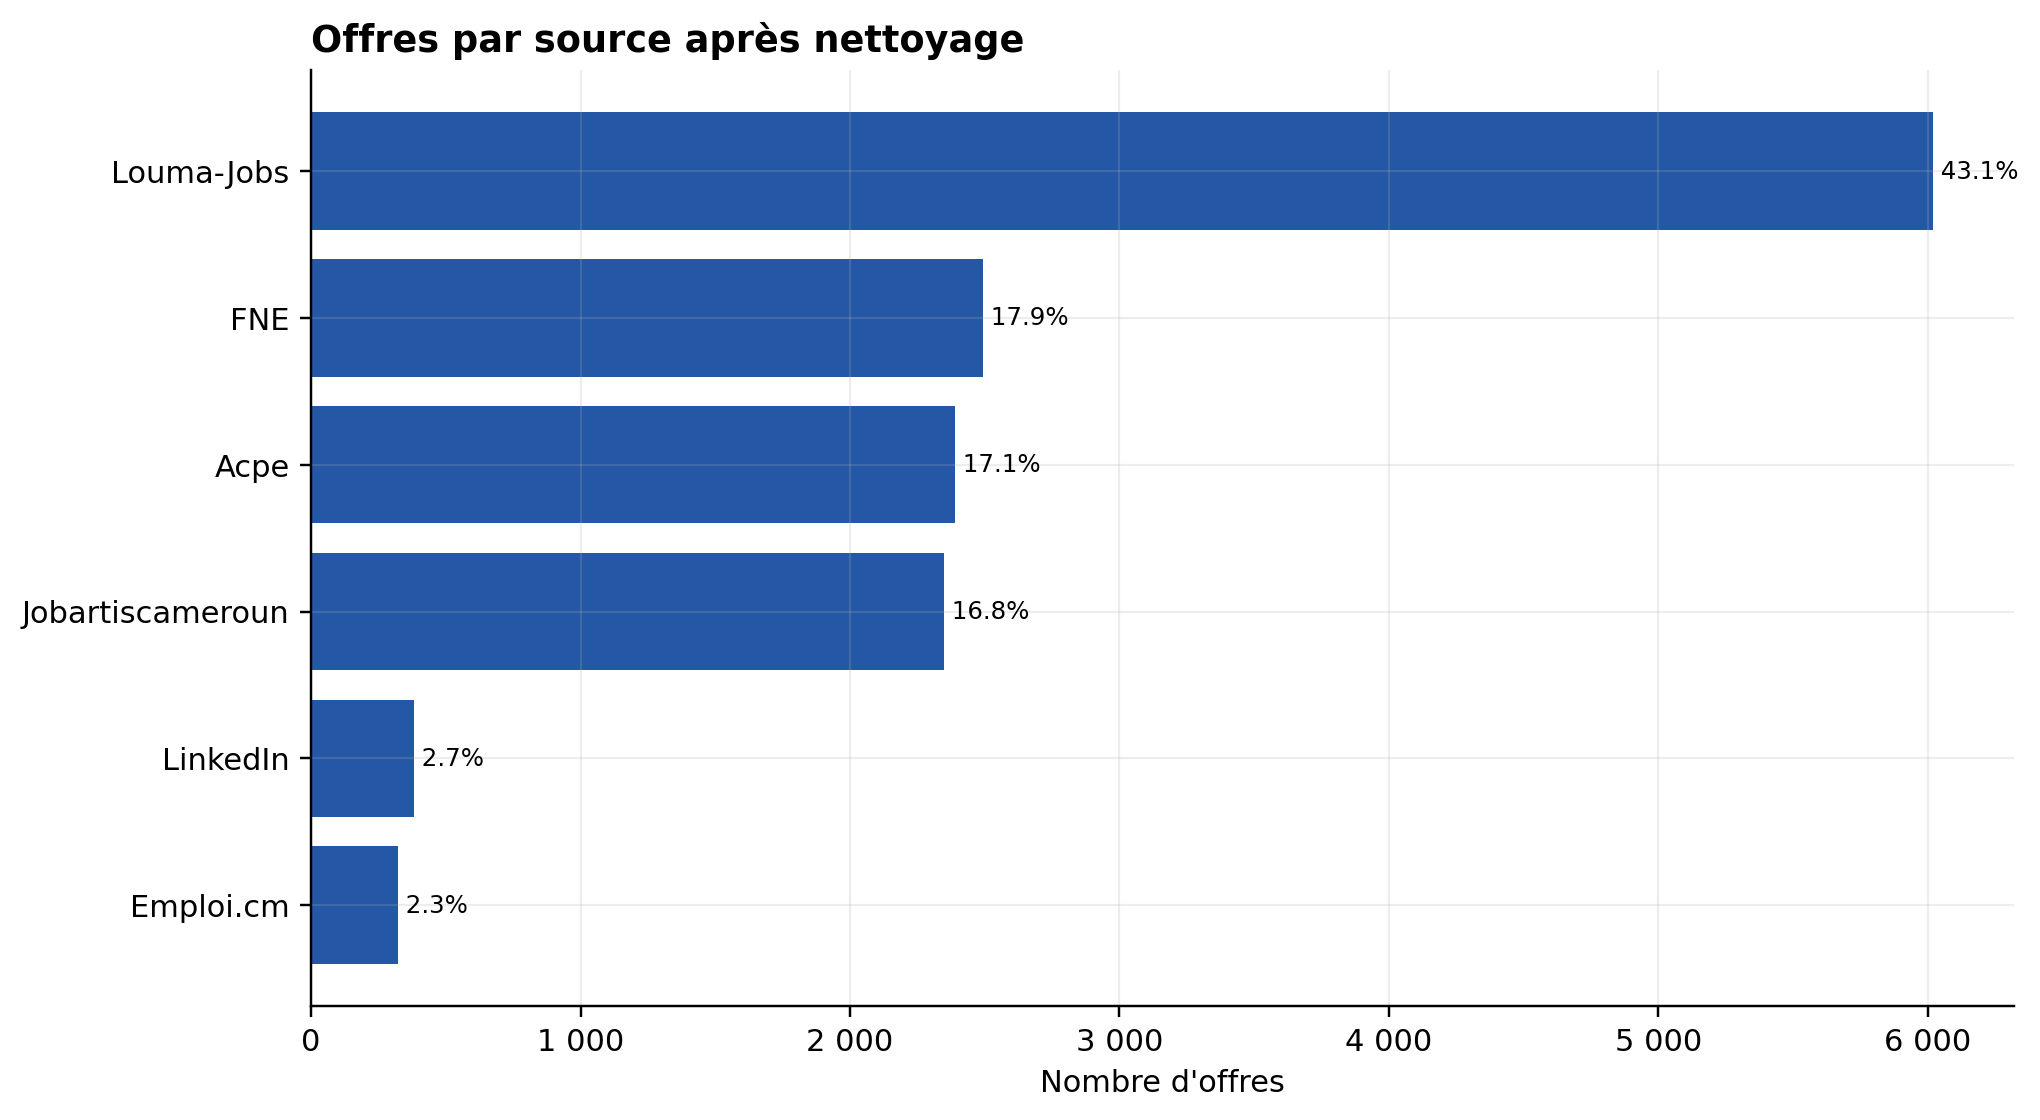
\includegraphics[width=0.86\textwidth]{figures/generated/implementation_deep_current/01_offres_par_source.png}
  \source{Nos travaux, traitements Python de nettoyage et de diagnostic, à partir des données collectées du projet.}
\end{figure}

Les 13\,957 offres proviennent de sources hétérogènes, dont plusieurs ont été scrapées : Emploi.cm, Jobartis Cameroun, LinkedIn, Louma-Jobs, ainsi que les sources institutionnelles FNE et ACPE. Louma-Jobs domine le corpus avec 6\,021 offres, soit 43,14\,\%. Le corpus est donc exploitable pour un prototype opérationnel, mais il ne doit pas être présenté comme une photographie exhaustive du marché camerounais de l'emploi.

\subsection{Qualité des variables utiles au matching emploi-compétences}
La qualité utile au matching dépend surtout de six variables : description, compétences, localisation, secteur, niveau et source. Elles alimentent directement le champ \filevar{text\_to\_embed}, les filtres pgvector et les relations Neo4j. Le diagnostic reste donc ciblé : que peut-on utiliser sans inventer d'information ?

\subsubsection{Localisation exploitable pour filtrer sans exclure}
Le diagnostic détaillé de localisation est renvoyé en annexe (figure~\ref{fig:implementation_localisation}). Dans le corps du chapitre, on retient seulement que la localisation est suffisamment renseignée pour filtrer et expliquer les recommandations, mais pas assez homogène pour être utilisée comme contrainte dure.

La localisation est exploitable, mais seulement comme filtre souple : 79,88\,\% des offres sont rattachées au Cameroun et 20,12\,\% à l'international. Lorsque la ville manque mais que le pays existe, le nettoyage conserve le pays sans inventer une ville. Le système peut donc expliquer une recommandation par zone géographique, mais il ne doit pas exclure brutalement une offre parce que la ville est absente.

\subsubsection{Compétences et descriptions : signal utile mais hétérogène}

\begin{figure}[H]
  \centering
  \caption{Compétences fréquentes et disponibilité descriptive}
  \label{fig:implementation_competences_descriptions}
  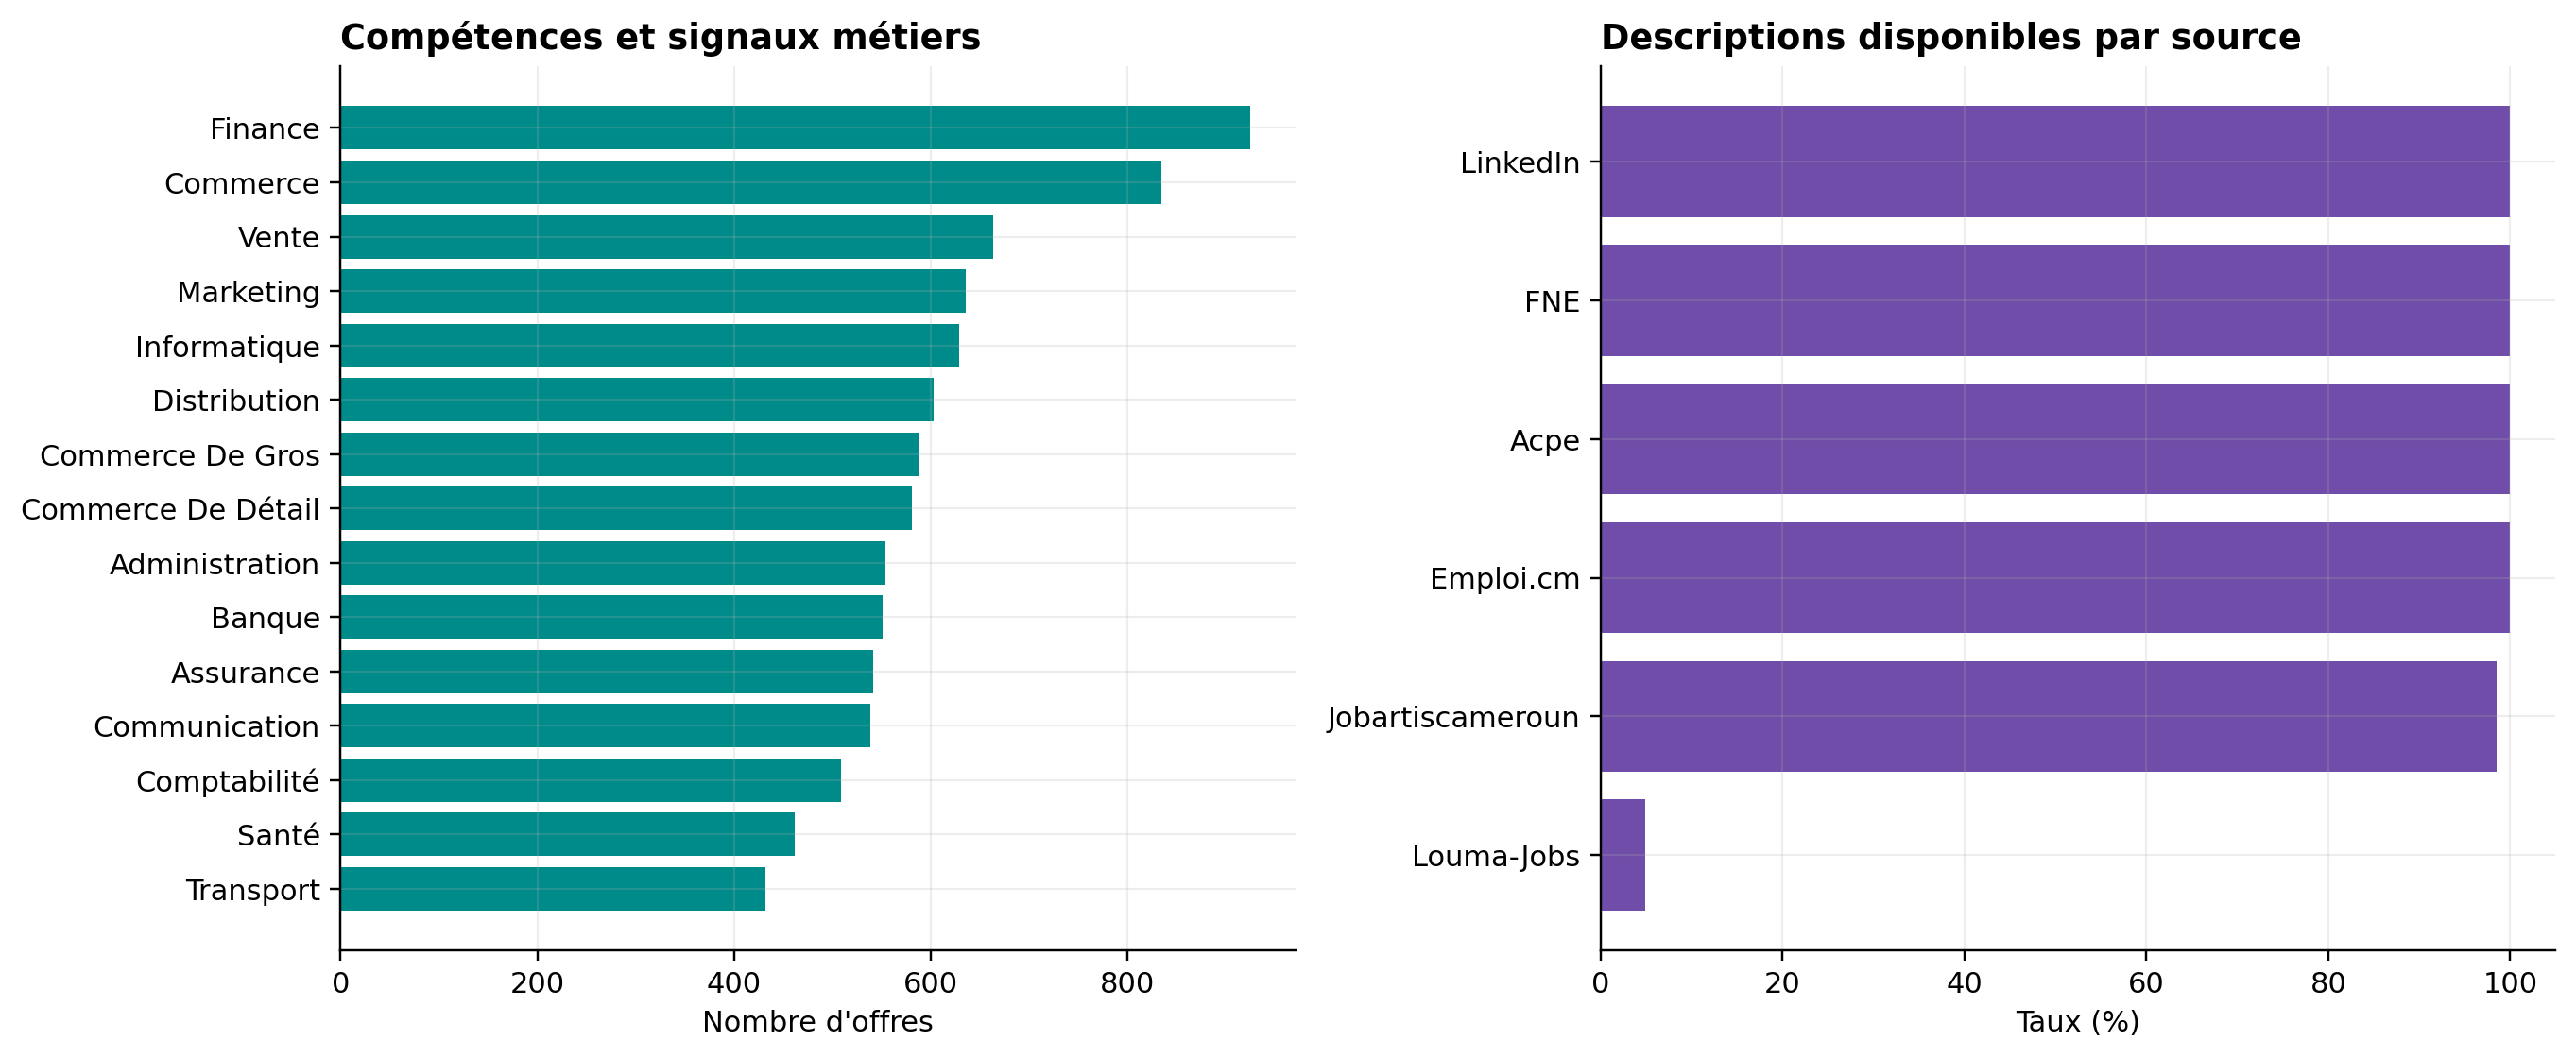
\includegraphics[width=0.94\textwidth]{figures/generated/implementation_deep_current/03_competences_descriptions.png}
  \source{Nos travaux, traitements Python de nettoyage et de diagnostic, à partir des données collectées du projet.}
\end{figure}

Les signaux les plus fréquents sont Finance, Commerce, Vente, Marketing, Informatique, Distribution, Banque, Assurance, Communication, Comptabilité, Santé et Transport. Cette structure est cohérente avec un système emploi--compétences, mais elle révèle un risque méthodologique : plusieurs libellés sont des domaines d'activité plutôt que des compétences observables. Dans l'implémentation, ces variables sont donc utilisées comme signaux d'appariement et de contexte, non comme preuve définitive d'une compétence maîtrisée par un candidat.

La disponibilité descriptive est le principal point faible du corpus. Les sources FNE, ACPE, LinkedIn et Emploi.cm disposent d'une description pour toutes leurs offres dans le fichier nettoyé ; Jobartis Cameroun atteint 98,55\,\%. La limite vient de Louma-Jobs : seulement 295 descriptions disponibles sur 6\,021 offres, soit 4,90\,\%. Cette hétérogénéité explique un choix central de l'ETL : la représentation envoyée au modèle d'embeddings ne peut pas être uniquement le détail textuel de l'offre ; elle doit combiner métadonnées, compétences, secteur, localisation et description lorsque celle-ci existe.

\subsection{Nettoyage réalisé et limites conservées}

Le nettoyage suit une règle conservatrice : corriger les formats sans fabriquer une information absente. Les libellés sont harmonisés, les localisations sont normalisées par priorité ville puis pays, et les doublons ne sont supprimés que lorsque la ligne normalisée est strictement identique. Ce choix protège le corpus multi-sources : deux offres peuvent avoir le même intitulé tout en différant par la ville, la source, le secteur, le niveau ou la description.

Le tableau détaillé des règles de nettoyage est placé en annexe (tableau~\ref{tab:implementation_nettoyage_donnees}). Le chapitre conserve uniquement le principe d'ingénierie : corriger les formats sans inventer une information absente des données brutes.

Les graphiques secondaires détaillant la structure sectorielle, les villes détaillées, les niveaux NCF, l'expérience, la structure des candidats, les longueurs de textes et les référentiels MEPC--NCF sont renvoyés en annexes. Dans ce chapitre, seuls les résultats qui changent une décision d'architecture sont conservés : enrichir les embeddings, utiliser pgvector pour le rappel rapide, exploiter Neo4j pour les contraintes métier, et garder un critic pour contrôler les réponses générées.

\section{Adaptation du modèle d'embeddings au domaine emploi--compétences}

Dans le workflow méthodologique, cette section correspond à l'étape située après l'ETL et avant l'indexation pgvector. Les données nettoyées sont transformées en paires d'apprentissage, puis l'encodeur SentenceTransformer est adapté au vocabulaire emploi--compétences. Le résultat attendu n'est pas une réponse générée, mais un encodeur capable de produire des vecteurs plus utiles pour le retrieval.

\subsection{Encodeur retenu et paires contrastives}

Le modèle de base retenu est \texttt{sentence-transformers/all-MiniLM-L6-v2}. Ce choix est défendable pour une raison d'ingénierie : il produit des embeddings de 384 dimensions, donc moins coûteux à stocker et à rechercher que des modèles à 768 dimensions, tout en restant compatible avec une indexation HNSW dans pgvector. Dans ce projet, la contrainte est concrète : le même encodeur sert ensuite à vectoriser les candidats, les offres, les compétences, les métiers et les référentiels. Un modèle plus lourd peut améliorer certains cas sémantiques, mais il augmente la taille de stockage, la latence d'encodage et le coût de réindexation.

Ce modèle est acceptable comme point de départ parce qu'il fournit déjà une représentation dense générale des phrases. Il n'est toutefois pas suffisant comme modèle final. Un encodeur généraliste rapproche des textes proches en langage courant, mais il ne connaît pas nécessairement les proximités utiles au domaine emploi-compétences camerounais : intitulés locaux, secteurs, niveaux de formation, familles métiers, descriptions incomplètes et compétences parfois formulées comme domaines. Le fine-tuning vise donc à spécialiser l'espace vectoriel sans changer l'architecture de production.

\begin{table}[H]
  \centering
  \caption{Protocole de construction des paires de fine-tuning}
  \label{tab:implementation_protocole_finetuning}
  \tableStyleStart
  \begin{tabularx}{\textwidth}{p{3.5cm}X}
    \rowcolor{darkblue}
    \tabheader{Élément} & \tabheader{Implémentation observée} \\
    \midrule
    Modèle de départ & \texttt{sentence-transformers/all-MiniLM-L6-v2}, embeddings denses de 384 dimensions. \\
    Rôle de \texttt{sentence1} & Représentation structurée de l'offre : titre, secteur, contrat, niveau d'études, expérience, ville et compétences. \\
    Rôle de \texttt{sentence2} & Détails nettoyés de l'annonce uniquement, c'est-à-dire le texte descriptif que le modèle doit rapprocher de la représentation structurée. \\
    Filtrage informatif & Conservation des paires avec compétences disponibles, \texttt{sentence1} d'au moins 40 caractères et \texttt{sentence2} d'au moins 120 caractères ; le champ \texttt{ft\_eligible} est appliqué lorsqu'il existe. \\
    Nombre total de paires & 6\,476 paires offre--description. \\
    Split & 4\,542 paires en train, 981 en validation et 953 en test, avec stratification par secteur principal. \\
    %Fichiers produits & \filevar{data/finetune/pairs\_train.jsonl}, \filevar{pairs\_val.jsonl}, \filevar{pairs\_test.jsonl} et \filevar{pairs\_metadata.json}. \\
    \bottomrule
  \end{tabularx}
  \tableStyleEnd
  \source{Nos travaux, traitements Python et SentenceTransformer, à partir des paires emploi--compétences et des entités nettoyées du projet.}
\end{table}

La structure \texttt{sentence1}/\texttt{sentence2} est volontairement asymétrique. \texttt{sentence1} représente la requête métier structurée que le système manipulera souvent en production : métadonnées, compétences et contexte de l'offre. \texttt{sentence2} représente le texte descriptif à retrouver. Ce choix entraîne le modèle à rapprocher une description naturelle d'une formulation structurée, ce qui correspond mieux au besoin du système qu'un entraînement sur deux phrases descriptives ordinaires.

Le filtrage des offres informatives est nécessaire. Entraîner le modèle sur des paires dont la description est vide, trop courte ou sans compétences introduirait du bruit : le modèle apprendrait à rapprocher des textes pauvres au lieu de structurer le domaine. Le seuil de 120 caractères pour \texttt{sentence2} et de 40 caractères pour \texttt{sentence1} est donc un garde-fou d'apprentissage. Il réduit le volume utilisé pour le fine-tuning, mais améliore la qualité du signal.
\subsection{Fine-tuning : contraintes de calcul et preuve de gain}

\subsubsection{Paramétrage contraint et dynamique d'apprentissage}

\begin{table}[H]
  \centering
  \caption{Hyperparamètres du fine-tuning SentenceTransformer}
  \label{tab:implementation_hyperparametres_finetuning}
  \tableStyleStart
  \begin{tabularx}{0.94\textwidth}{p{5.2cm}X}
    \rowcolor{darkblue}
    \tabheader{Hyperparamètre} & \tabheader{Valeur} \\
    \midrule
    Nombre d'époques & 5 \\
    Batch size & 32 \\
    Négatifs implicites par exemple & 31 \\
    Learning rate maximal & $2\times10^{-5}$ \\
    Scheduler & Cosine avec warmup \\
    Warmup & 100 étapes configurées, limitées par les étapes disponibles de l'époque \\
    Perte & \textit{MultipleNegativesRankingLoss} avec similarité cosinus \\
    Temps d'entraînement observé & 15\,160 s \\
    Checkpoint retenu & Meilleur checkpoint sur validation autour de l'époque 4 \\
    \bottomrule
  \end{tabularx}
  \tableStyleEnd
  \source{Nos travaux, traitements Python de nettoyage et de diagnostic, à partir des données collectées du projet.}
\end{table}

Ces hyperparamètres ne sont pas des valeurs arbitraires. Ils traduisent un compromis imposé par les ressources disponibles : le fine-tuning devait rester exécutable localement, sans infrastructure GPU lourde ni entraînement long. Le modèle \texttt{all-MiniLM-L6-v2} a donc été conservé parce qu'il produit des vecteurs de 384 dimensions, moins coûteux à encoder, stocker et rechercher dans pgvector. Le batch de 32 limite la consommation mémoire tout en conservant assez d'exemples négatifs implicites pour la \textit{MultipleNegativesRankingLoss}. Le nombre de cinq époques évite un entraînement excessif sur un corpus de paires encore imparfait. Le \textit{learning rate} de $2\times10^{-5}$, avec \textit{warmup} puis décroissance, permet une adaptation progressive du modèle sans déstabiliser les représentations déjà apprises.

\begin{figure}[H]
  \centering
  \caption{Diagnostic du fine-tuning : perte, généralisation, métriques de validation et calendrier du learning rate}
  \label{fig:implementation_finetuning_courbes}
  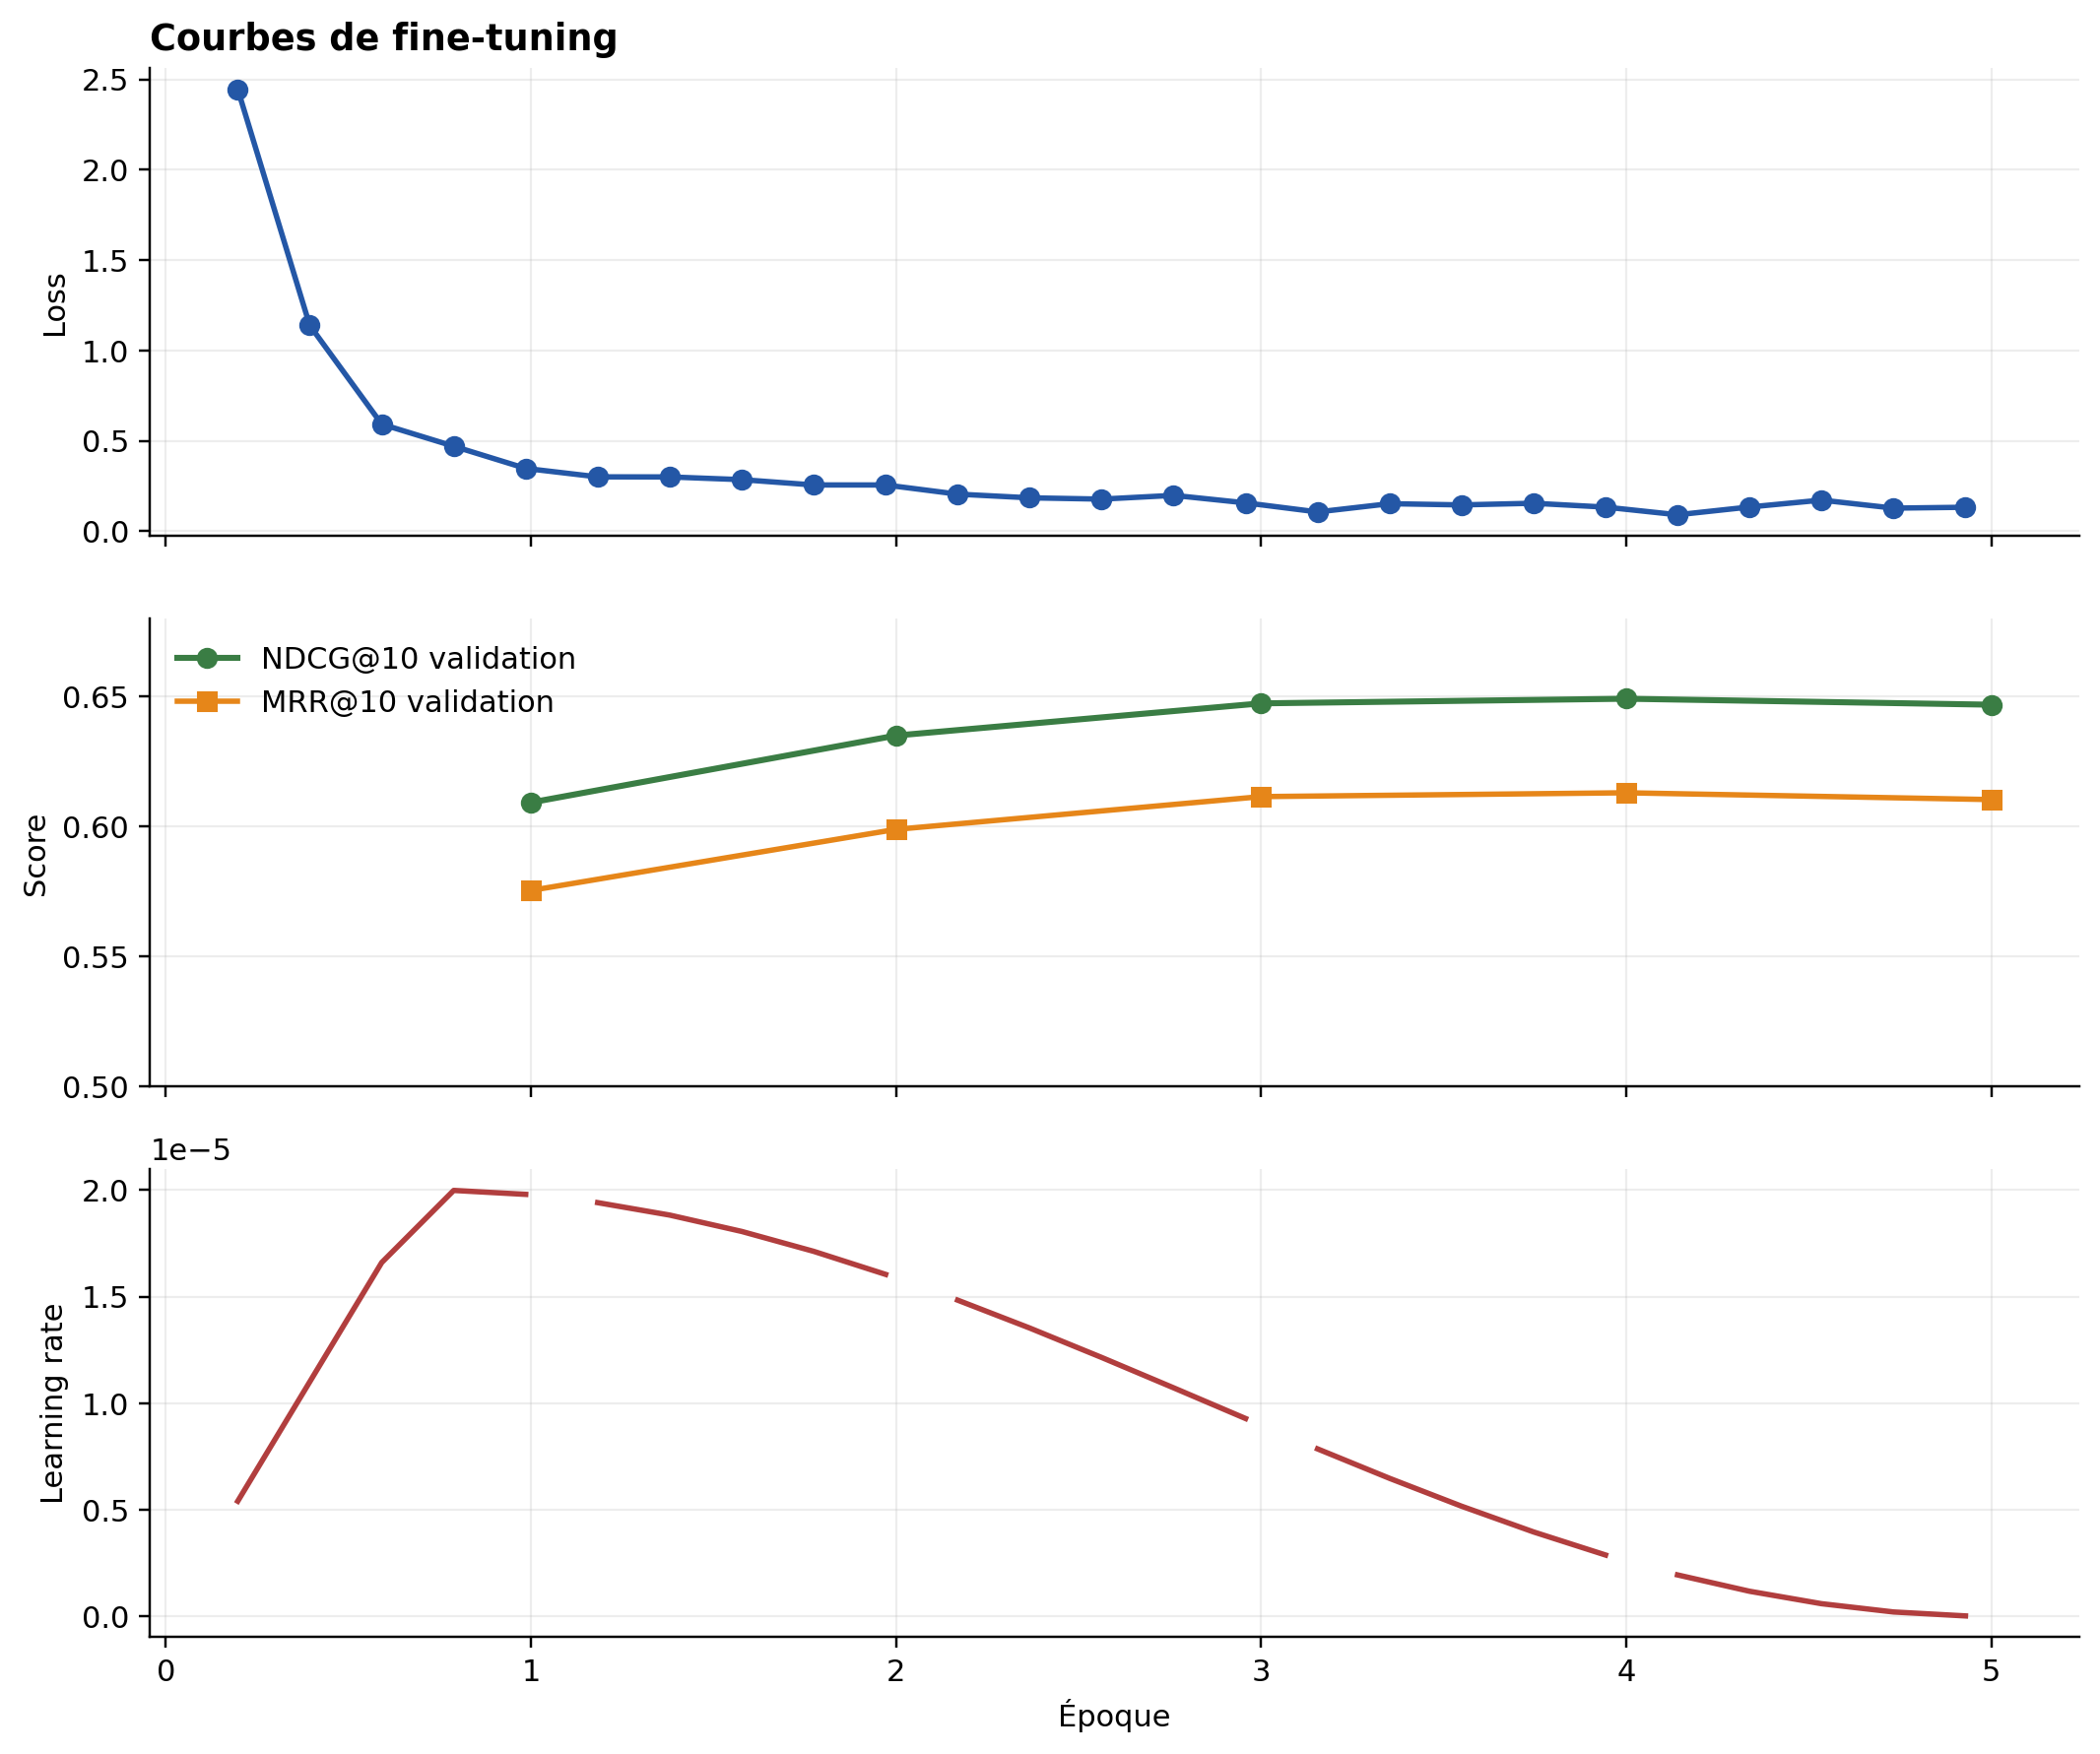
\includegraphics[width=0.92\textwidth]{figures/generated/implementation_deep_current/04_finetuning_courbes.png}
  \source{Nos travaux, traitements Python et SentenceTransformer, à partir des paires emploi--compétences et des entités nettoyées du projet.}
\end{figure}

La figure \ref{fig:implementation_finetuning_courbes} se lit en quatre blocs. Le premier montre que la perte d'entraînement chute fortement au début, de 2,445 à 0,132 en fin d'entraînement : le modèle apprend rapidement à rapprocher les paires positives du domaine. Le deuxième bloc compare la perte finale sur un échantillon fixe de 64 paires par split : 0,171 sur train, 0,285 sur validation et 0,433 sur test. Cette hausse est normale : les jeux non vus sont plus difficiles que les exemples utilisés pendant l'apprentissage. Le troisième bloc montre que les métriques de validation progressent jusqu'aux dernières époques, avec un léger tassement final ; il n'y a donc pas de signal évident d'effondrement. Le quatrième bloc rappelle le choix de ressources : un \textit{learning rate} maximal de $2\times10^{-5}$, 100 étapes de \textit{warmup}, un batch de 32 et seulement cinq époques. Le protocole cherche donc un gain utile de classement, pas une optimisation coûteuse et difficile à reproduire.

Ces valeurs ne remplacent pas les métriques de ranking, car la \textit{MultipleNegativesRankingLoss} dépend de la composition des batches. Elles servent surtout de contrôle de cohérence : si la perte train baissait mais que la validation stagnait ou chutait, le fine-tuning serait suspect. Ici, la baisse de perte et la progression du NDCG@10/MRR@10 indiquent que l'adaptation du modèle améliore bien le retrieval dans le domaine emploi--compétences.

La validation atteint un NDCG@10 maximal de 0,6492 à l'époque 4, avant un léger recul à 0,6469 à l'époque 5. Ce profil est cohérent avec un apprentissage rapide suivi d'un plateau. Il serait donc fragile de prolonger l'entraînement sans contrôle : au-delà d'un certain point, le gain marginal devient faible et le risque de sur-adaptation augmente.

\subsubsection{Preuve de gain sur le ranking sémantique}

La comparaison numérique directe entre baseline et modèle fine-tuné est reportée en annexe (tableau~\ref{tab:implementation_baseline_vs_finetuned}), tandis que l'évaluation complète du retrieval est reprise au chapitre~4.

Cette comparaison a été régénérée sur 953 paires de test après la mise à jour du jeu de paires. Elle est la preuve la plus directe de l'intérêt du fine-tuning : le modèle de base ne structure pas correctement le domaine dans ce protocole, alors que le modèle adapté récupère beaucoup plus souvent la description pertinente dans les premiers rangs. Le NDCG@10 est multiplié par 3,7 et le MRR@10 par 4,2. Le gain de recall@10 est particulièrement important, car l'application ne dépend pas d'une seule réponse immédiate ; elle récupère d'abord un ensemble court de candidats pertinents avant reranking hybride.

\begin{figure}[H]
  \centering
  \caption{Comparaison des modèles d'embeddings : qualité de classement, rappel et latence}
  \label{fig:implementation_benchmark_embeddings}
  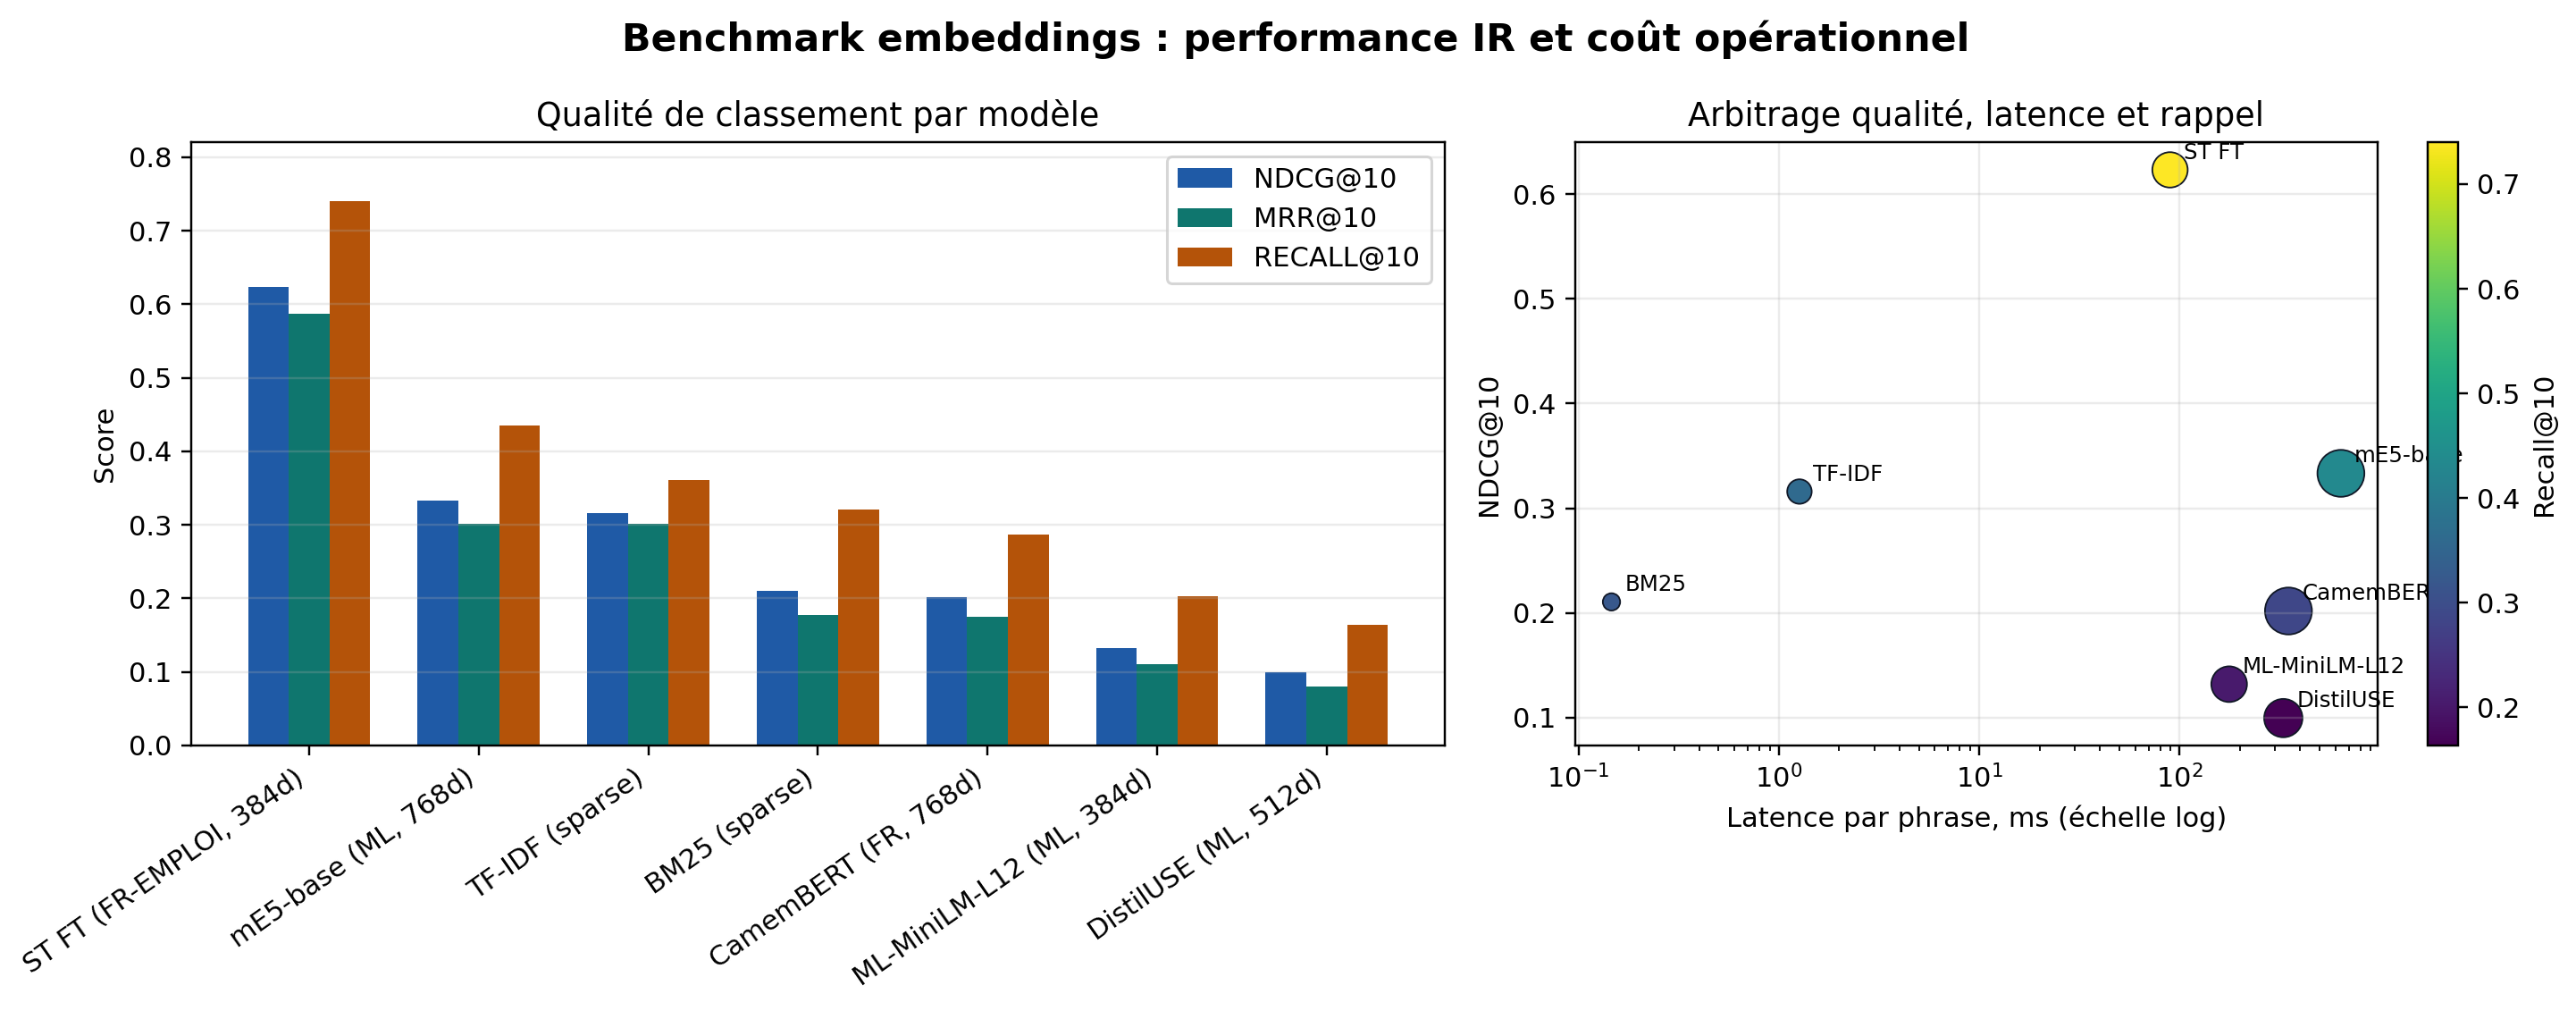
\includegraphics[width=0.92\textwidth]{figures/generated/implementation_deep_current/05_benchmark_modeles_embeddings.png}
  \source{Nos travaux, traitements Python et SentenceTransformer, à partir des paires emploi--compétences et des entités nettoyées du projet.}
\end{figure}

Le benchmark multi-modèles confirme le résultat. Le modèle fine-tuné atteint un NDCG@10 de 0,6232, un MRR@10 de 0,5874 et un recall@10 de 0,7398. Le meilleur modèle généraliste dense testé, mE5-base, atteint seulement 0,3333 en NDCG@10 et 0,4355 en recall@10, avec une latence nettement plus élevée. TF-IDF reste très rapide et compétitif sur certains signaux lexicaux, mais son recall@10 reste inférieur à celui du modèle fine-tuné. L'intérêt du fine-tuning est donc empirique, pas seulement théorique. La bonne architecture n'oppose pas \og deep learning \fg{} et lexical ; elle utilise le modèle fine-tuné comme signal sémantique principal et conserve les signaux lexicaux comme complément.

\subsection{Structure de l'espace vectoriel après fine-tuning}

\begin{figure}[H]
  \centering
  \caption{Projection UMAP des embeddings indexés}
  \label{fig:implementation_espace_vectoriel}
  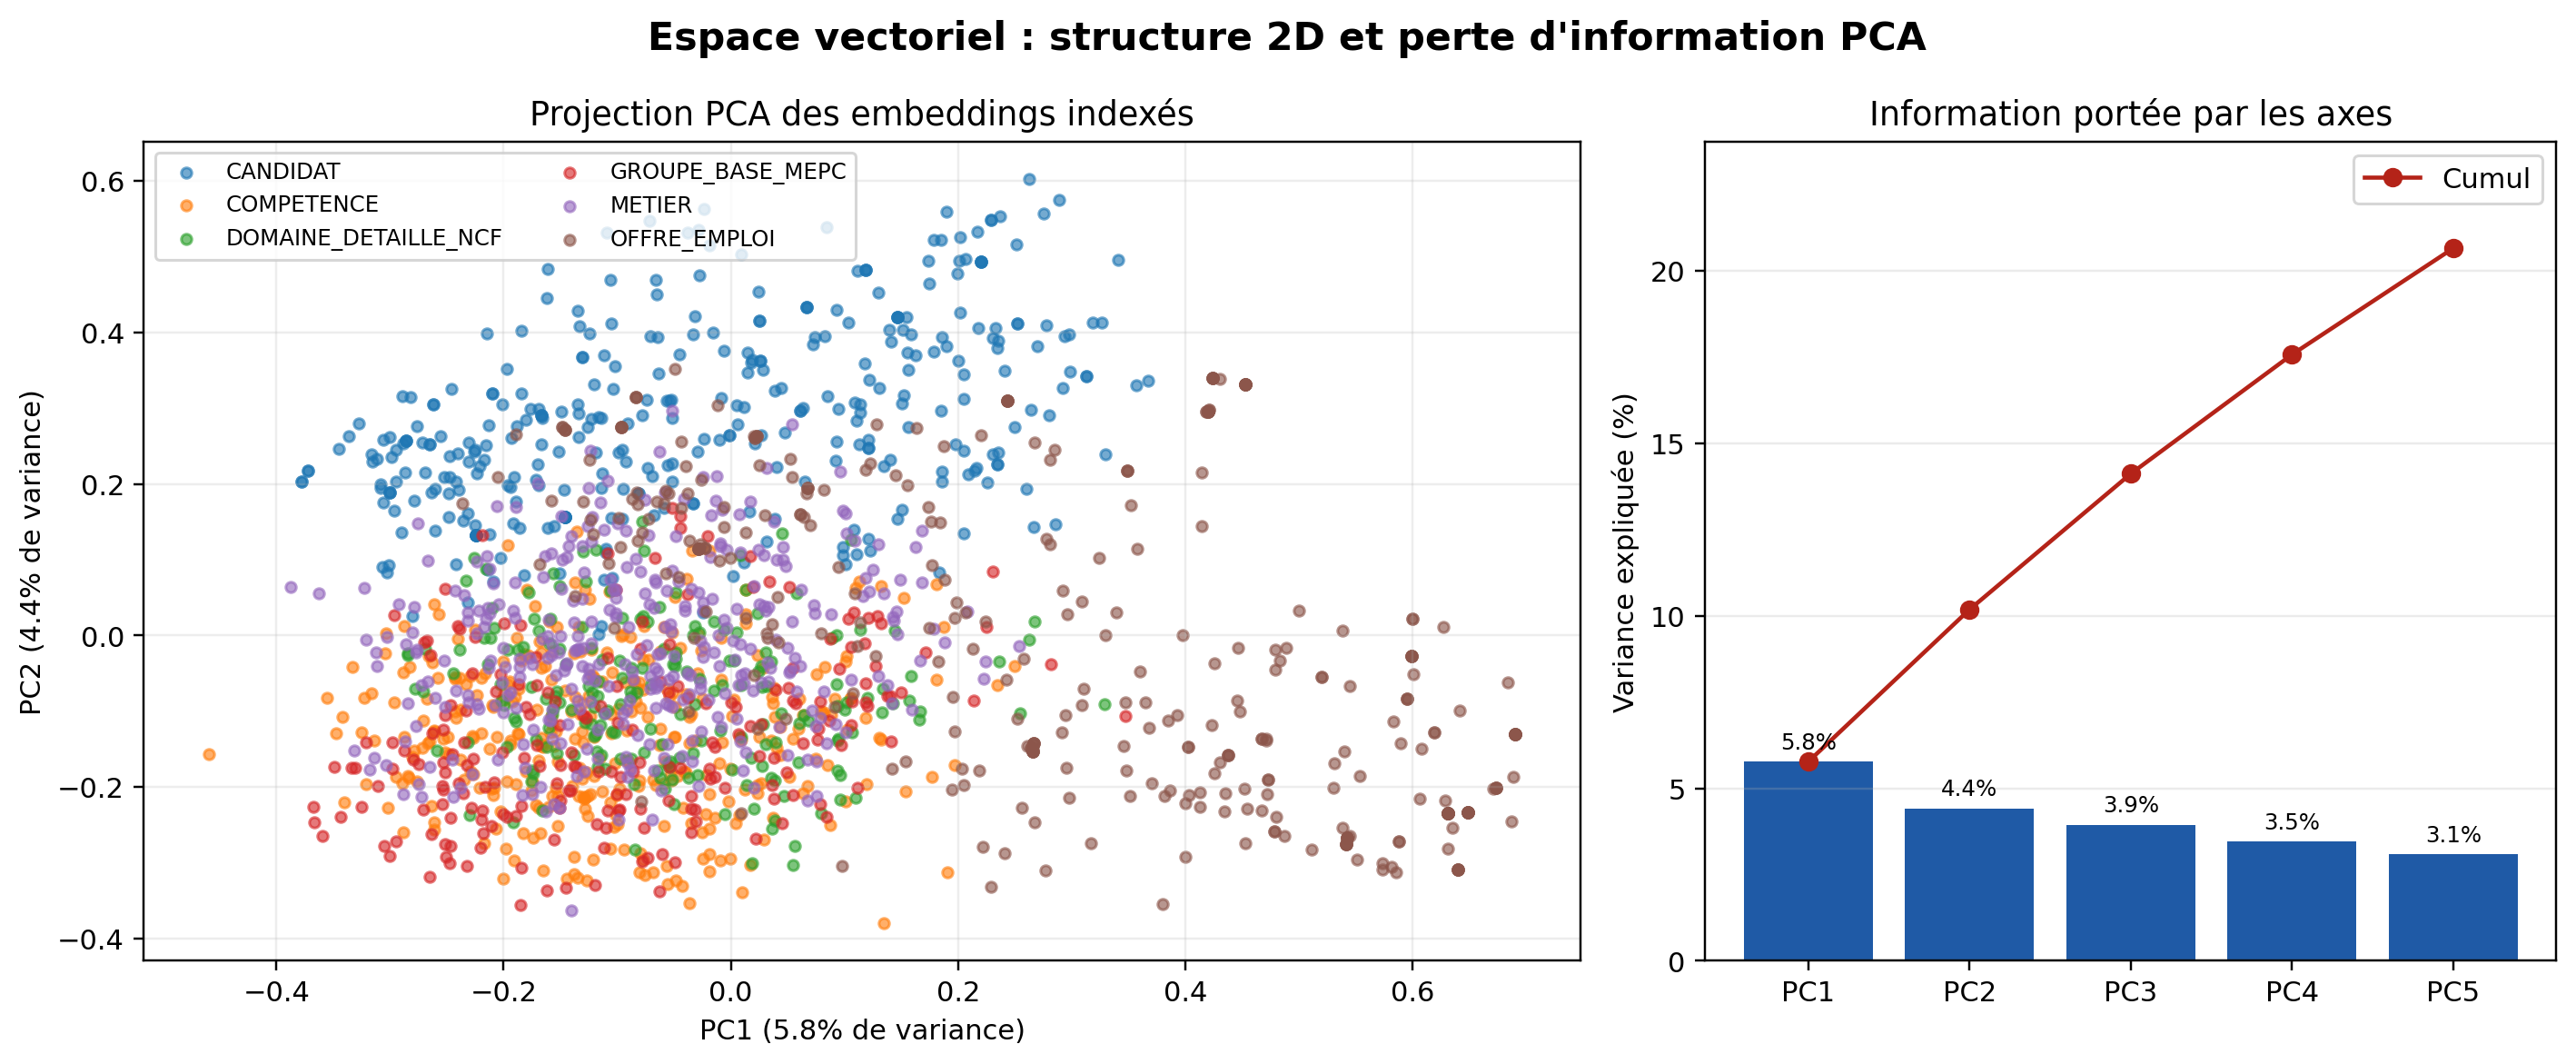
\includegraphics[width=0.94\textwidth]{figures/generated/implementation_deep_current/07_espace_vectoriel_embeddings.png}
  \source{Nos travaux, traitements Python et SentenceTransformer, à partir des paires emploi--compétences et des entités nettoyées du projet.}
\end{figure}

La figure \ref{fig:implementation_espace_vectoriel} utilise UMAP pour projeter en deux dimensions un échantillon de 1\,810 embeddings indexés : 350 candidats, 350 offres, 350 compétences, 350 métiers, 209 groupes de base MEPC et 201 domaines détaillés NCF. UMAP est ici un outil de lecture visuelle. 
La première lecture porte sur la séparation partielle des familles d'objets. Les offres d'emploi apparaissent plus excentrées, avec un centroïde situé dans une zone différente de celle des autres types d'entités. C'est cohérent avec leur contenu : une offre combine titre, secteur, contrat, localisation, niveau et description, donc un vocabulaire plus contextuel. Les candidats, compétences, métiers, groupes MEPC et domaines NCF sont davantage rapprochés dans la partie centrale du nuage. Cette proximité n'est pas un défaut. Le système a précisément besoin que ces objets partagent un espace commun : un candidat doit pouvoir être rapproché de compétences, de métiers et d'offres, sinon pgvector ne pourrait pas servir de premier étage de retrieval.

La deuxième lecture concerne le recouvrement entre catégories. Le nuage ne montre pas des blocs parfaitement séparés, et il ne faut pas chercher cette séparation. Dans un système emploi--compétences, une compétence, un métier et un profil candidat peuvent partager les mêmes termes : \og comptabilité \fg{}, \og vente \fg{}, \og marketing \fg{}, \og informatique \fg{}. Le recouvrement visuel signifie donc que le modèle place dans une même région des objets qui parlent du même domaine, même s'ils n'ont pas le même type technique dans la base. C'est utile pour récupérer des voisins sémantiques ; c'est aussi la raison pour laquelle Neo4j reste nécessaire ensuite, car pgvector rapproche les textes mais ne vérifie pas à lui seul les relations \texttt{POSSEDE}, \texttt{REQUIERT} ou \texttt{NECESSITE}.

La visualisation doit enfin être lue avec discipline. UMAP ne prouve pas que les recommandations sont bonnes et ne remplace pas le benchmark. Il sert à vérifier que l'espace vectoriel n'est pas incohérent : les offres ne sont pas mélangées au hasard, les objets référentiels restent raccordés aux profils et aux compétences, et les zones mixtes rendent possible la recherche sémantique. La preuve quantitative reste le ranking présenté en section précédente, notamment le NDCG@10, le MRR@10 et le recall@10.

%\begin{figure}[H]
%  \centering
%  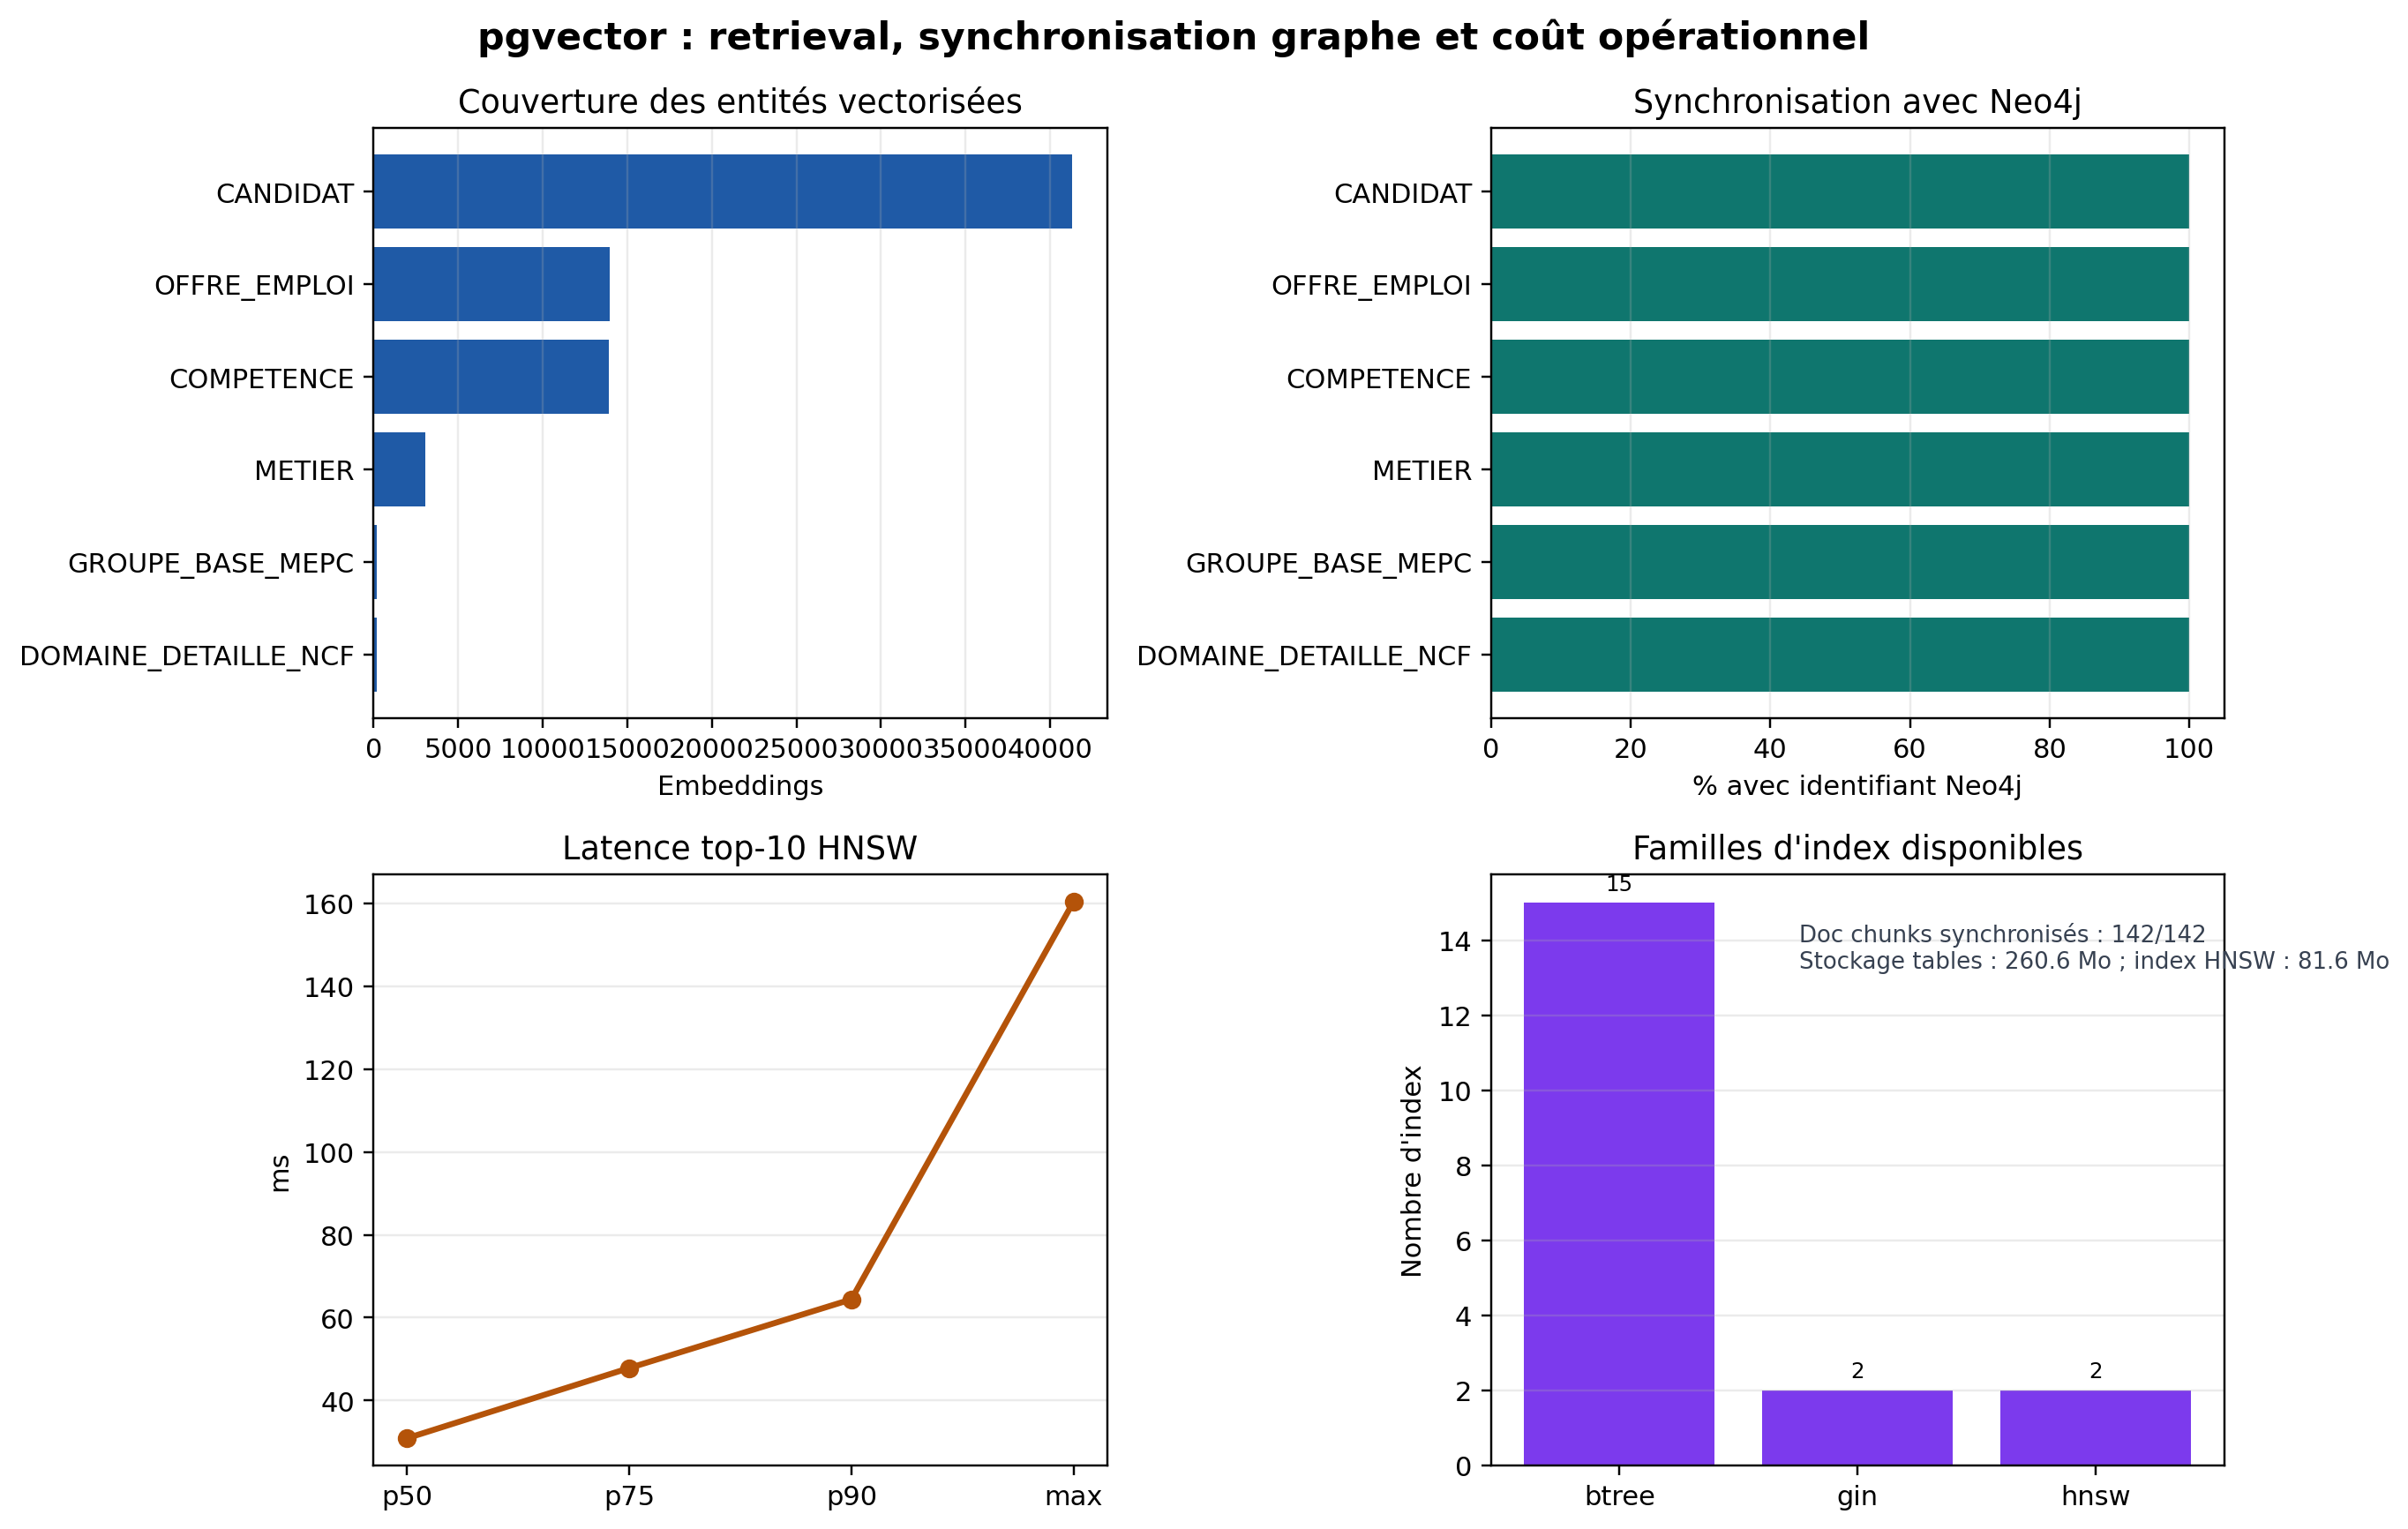
\includegraphics[width=0.94\textwidth]{figures/generated/implementation_deep_current/06_pgvector_retrieval_dashboard.png}
%  \caption{Dashboard pgvector : couverture, synchronisation graphe, latence et index}
%  \label{fig:implementation_pgvector_retrieval_dashboard}
 % \source{\texttt{06\_pgvector\_counts.csv}, \texttt{06\_pgvector\_latency\_summary.csv}, \texttt{06\_pgvector\_sizes.csv}, \texttt{06\_pgvector\_indexes.csv} et \texttt{06\_pgvector\_doc\_chunks.csv}}
%\end{figure}

%Ce graphique ne répète pas seulement les volumes du tableau suivant. Il donne quatre informations opérationnelles différentes : la taille du vivier vectorisé, la capacité à rejoindre Neo4j, la latence du top-10 HNSW et les familles d'index disponibles. La lecture est simple : pgvector couvre les entités utiles, toutes sont raccordables au graphe, la médiane de recherche reste autour de 31 ms, mais le maximum observé rappelle qu'une application interactive doit surveiller les cas lents. Le graphique sert donc à juger la brique comme outil de retrieval, pas comme simple base de stockage.

\section{Mémoire vectorielle pgvector pour le retrieval}

Dans le workflow, pgvector intervient juste après l'encodage des entités par le modèle fine-tuné. Il constitue le premier étage du retrieval de l'Agentic RAG : transformer une requête, un profil ou un fragment documentaire en vecteur, récupérer rapidement un top-$K$ d'objets proches, puis transmettre ce vivier au moteur hybride et au graphe Neo4j. pgvector ne décide donc pas seul de la recommandation finale ; il fournit la liste de départ que le graphe va contrôler.

\subsection{Schéma physique, tables et volumes indexés}

\begin{figure}[H]
  \centering
  \caption{Schéma physique de la base pgvector : tables documentaires, embeddings et index de recherche}
  \label{fig:implementation_schema_pgvector}
  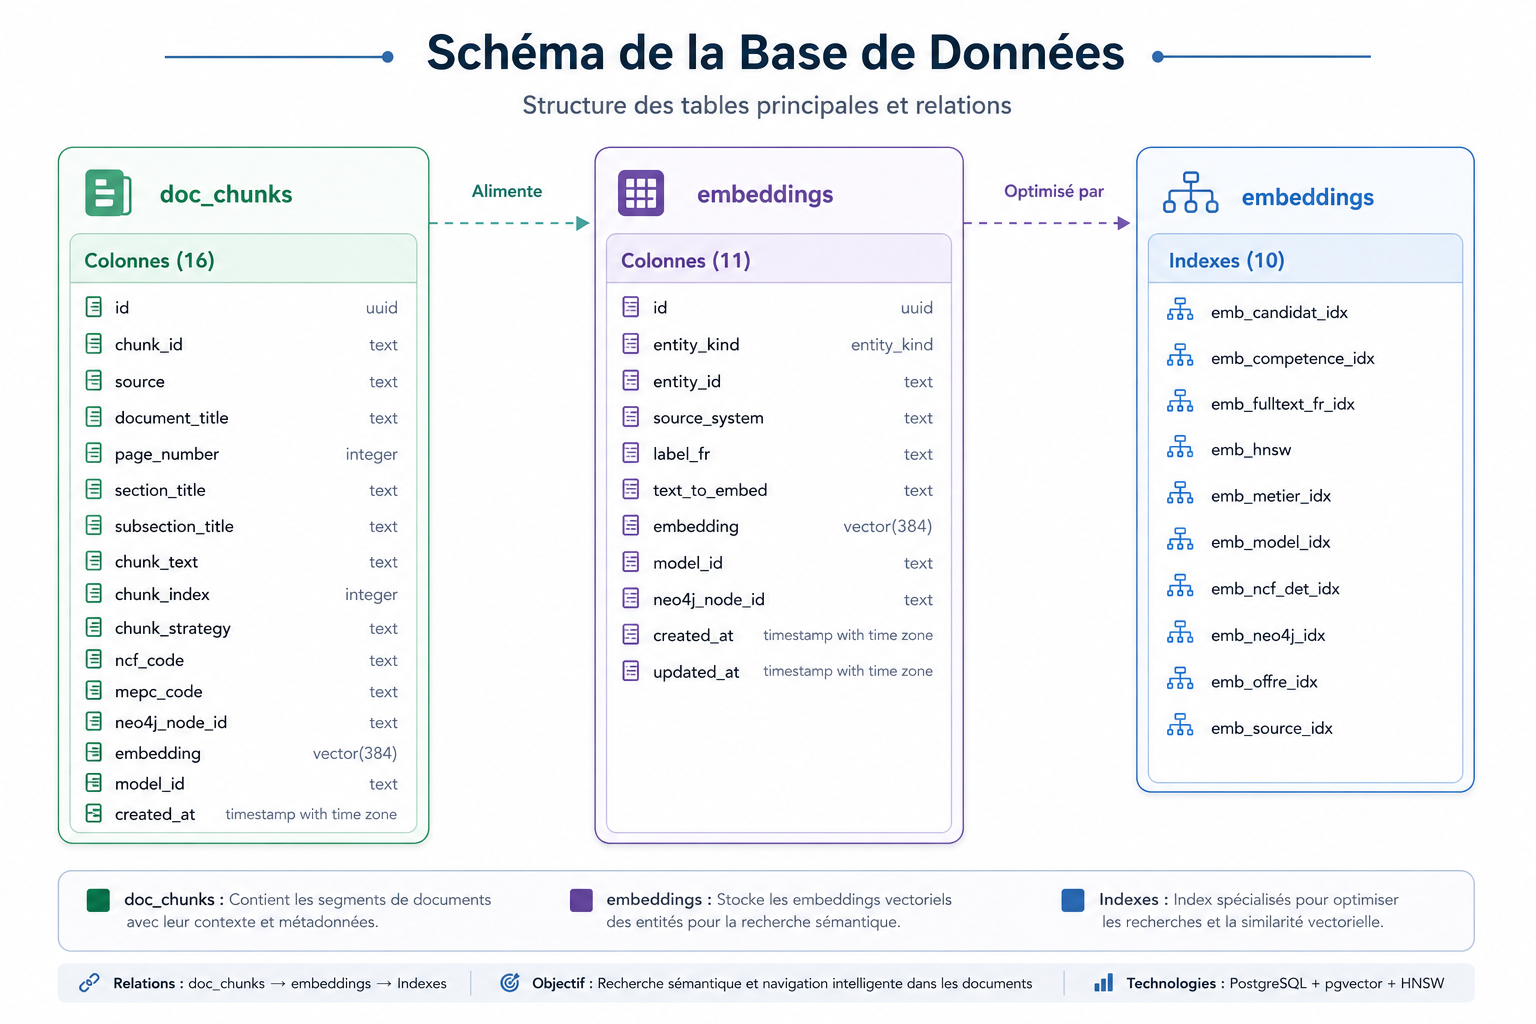
\includegraphics[width=0.96\textwidth]{pgvector.png}
  \source{Nos travaux, diagnostics PostgreSQL--pgvector}
\end{figure}

La figure \ref{fig:implementation_schema_pgvector} donne la lecture la plus simple de la brique pgvector. La table \texttt{embeddings} stocke les vecteurs des entités structurées : candidats, offres, compétences, métiers, groupes \MEPC{} et domaines \NCF{}. La table \texttt{doc\_chunks} stocke les fragments documentaires issus des référentiels. Les index spécialisés servent ensuite à interroger ces deux familles d'objets par similarité vectorielle, par recherche textuelle, par type d'entité, par modèle d'embedding ou par identifiant Neo4j.

Cette séparation évite une confusion fréquente : pgvector n'est pas seulement une colonne \texttt{vector}. C'est une couche de retrieval qui associe trois informations dans la même base : le vecteur, les métadonnées métier et le lien vers Neo4j. Le schéma suffit donc à comprendre les deux tables utiles : \texttt{embeddings} pour les entités structurées et \texttt{doc\_chunks} pour les fragments documentaires. Le détail technique des champs n'est pas répété ici, car l'image présente déjà la structure physique de la base.

Le modèle d'encodage utilisé est \texttt{all-MiniLM-L6-v2-ft-offres-cm}. Les vecteurs ont une dimension de 384, ce qui limite le coût de stockage et de recherche tout en restant adapté au retrieval sémantique. L'instance courante contient 72\,643 embeddings d'entités structurées et 142 embeddings documentaires, soit 72\,785 vecteurs interrogeables.

\begin{table}[H]
  \centering
  \caption{Distribution des embeddings par type d'entité}
  \label{tab:implementation_pgvector_distribution}
  \tableStyleStart
  \begin{tabularx}{0.92\textwidth}{Xrrr}
    \rowcolor{darkblue}
    \tabheader{Type d'entité} & \tabheader{Vecteurs} & \tabheader{Part} & \tabheader{Couverture Neo4j} \\
    \midrule
    Candidats & 41\,298 & 56,85\,\% & 100\,\% \\
    Offres d'emploi & 13\,957 & 19,22\,\% & 100\,\% \\
    Compétences & 13\,939 & 19,19\,\% & 100\,\% \\
    Métiers & 3\,039 & 4,18\,\% & 100\,\% \\
    Groupes de base MEPC & 209 & 0,29\,\% & 100\,\% \\
    Domaines détaillés NCF & 201 & 0,28\,\% & 100\,\% \\
    \midrule
    Total entités structurées & 72\,643 & 100\,\% & 100\,\% \\
    Chunks documentaires & 142 & -- & 100\,\% \\
    \bottomrule
  \end{tabularx}
  \tableStyleEnd
  \source{Nos travaux, diagnostics PostgreSQL--pgvector, à partir des embeddings, des métadonnées et des fragments documentaires indexés.}
\end{table}

Cette distribution montre que pgvector couvre les deux côtés du matching. Les candidats représentent 56,85\,\% des embeddings et les offres 19,22\,\%. Les compétences et métiers forment le vocabulaire pivot qui permet de relier une similarité textuelle à une logique emploi--compétences. La couverture Neo4j de 100\,\% est le point décisif : chaque résultat vectoriel peut être replacé dans le graphe pour récupérer secteur, niveau, localisation, compétences reliées ou chemin explicatif.

\subsection{Référentiels découpés en chunks interrogeables}

Les référentiels ne sont pas indexés comme de simples PDF. Ils sont d'abord découpés en fragments documentaires, puis chaque fragment reçoit un embedding et un identifiant Neo4j. Les documents référentiels ajoutent 142 chunks : 43 pour les diplômes, 61 pour le MEPC 2013 et 38 pour la NCF 2017. Cette double indexation est nécessaire au GraphRAG : pgvector retrouve le passage pertinent, puis Neo4j le rattache à une formation, un métier, un niveau ou un domaine.

La figure~\ref{fig:implementation_chunking_pipeline} situe précisément cette étape dans le workflow : documents sources, détection des titres, découpage structurel, validation des tailles, puis indexation dans \texttt{doc\_chunks}. La stratégie d'ingestion est structurelle par défaut. Elle détecte les titres de section à partir de la mise en forme et des motifs numérotés, puis chaque titre ouvre un chunk dont le contenu s'étend jusqu'au titre suivant. Les fragments de moins de 80 caractères sont fusionnés avec le fragment précédent et une limite supérieure de 3\,000 caractères contrôle la taille maximale. La stratégie sémantique de secours par fenêtres glissantes existe dans le pipeline, mais elle n'a pas été utilisée dans l'index courant : les 142 chunks proviennent tous du découpage structurel.

\begin{figure}[H]
  \centering
  \caption{Pipeline de chunking structurel des référentiels documentaires}
  \label{fig:implementation_chunking_pipeline}
  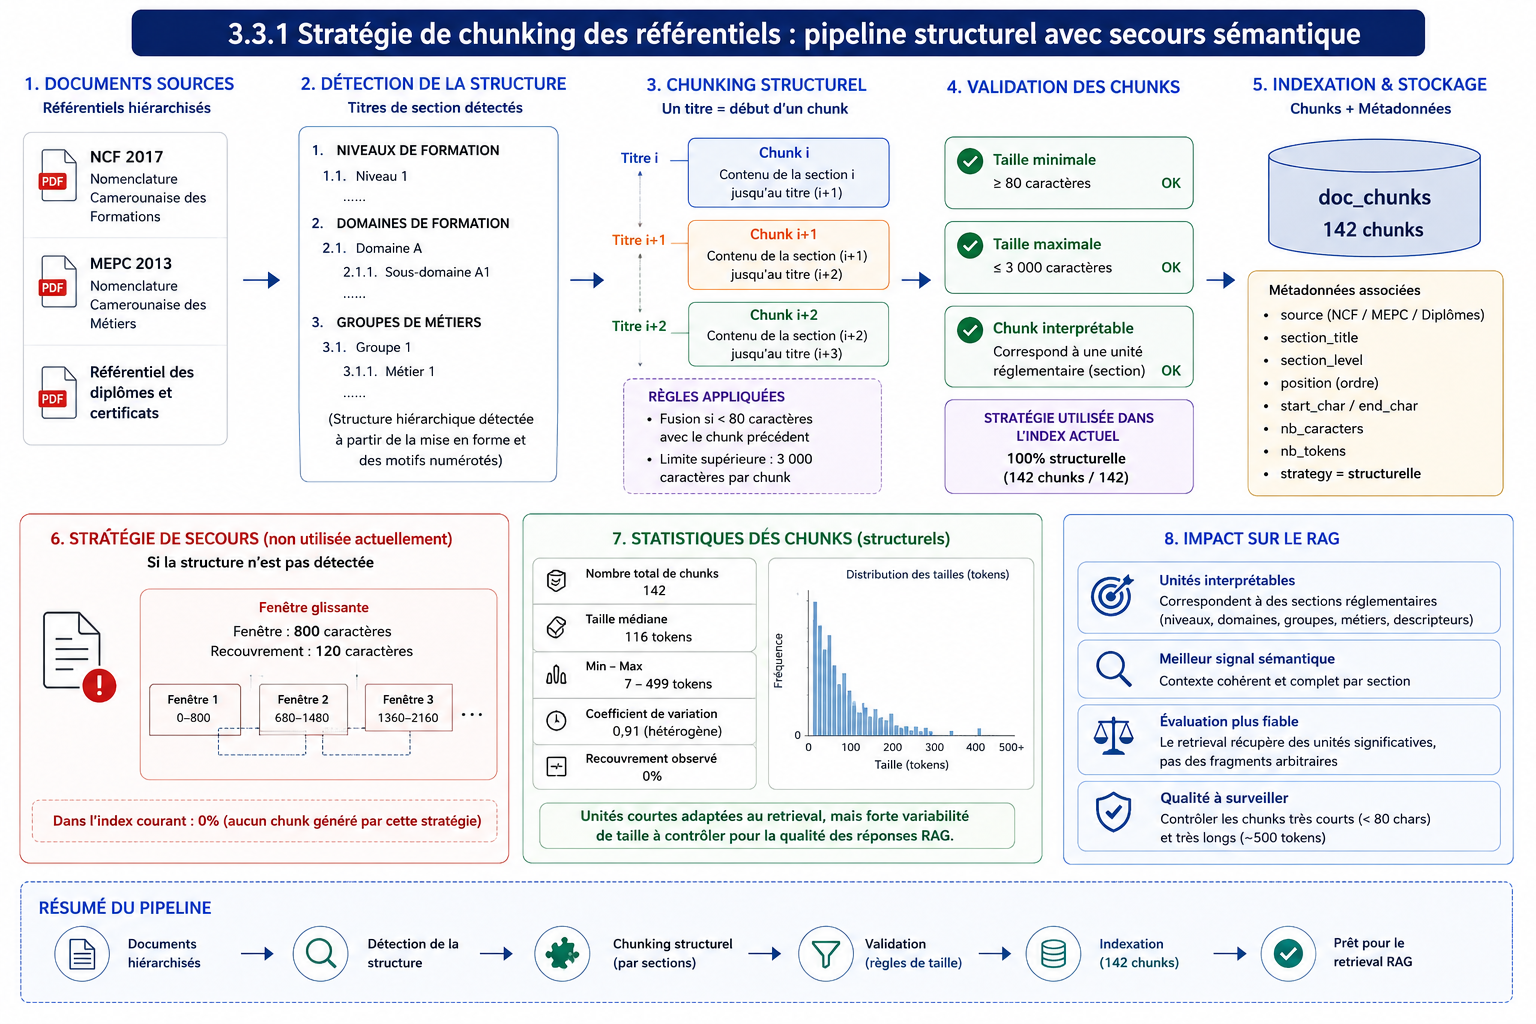
\includegraphics[width=0.96\textwidth]{chunking.png}
  \source{Nos travaux, schématisation du pipeline de chunking documentaire et d'indexation pgvector.}
\end{figure}

\begin{figure}[H]
  \centering
  \caption{Distribution des tailles, sources et couverture du chunking documentaire}
  \label{fig:implementation_chunking_diagnostics}
  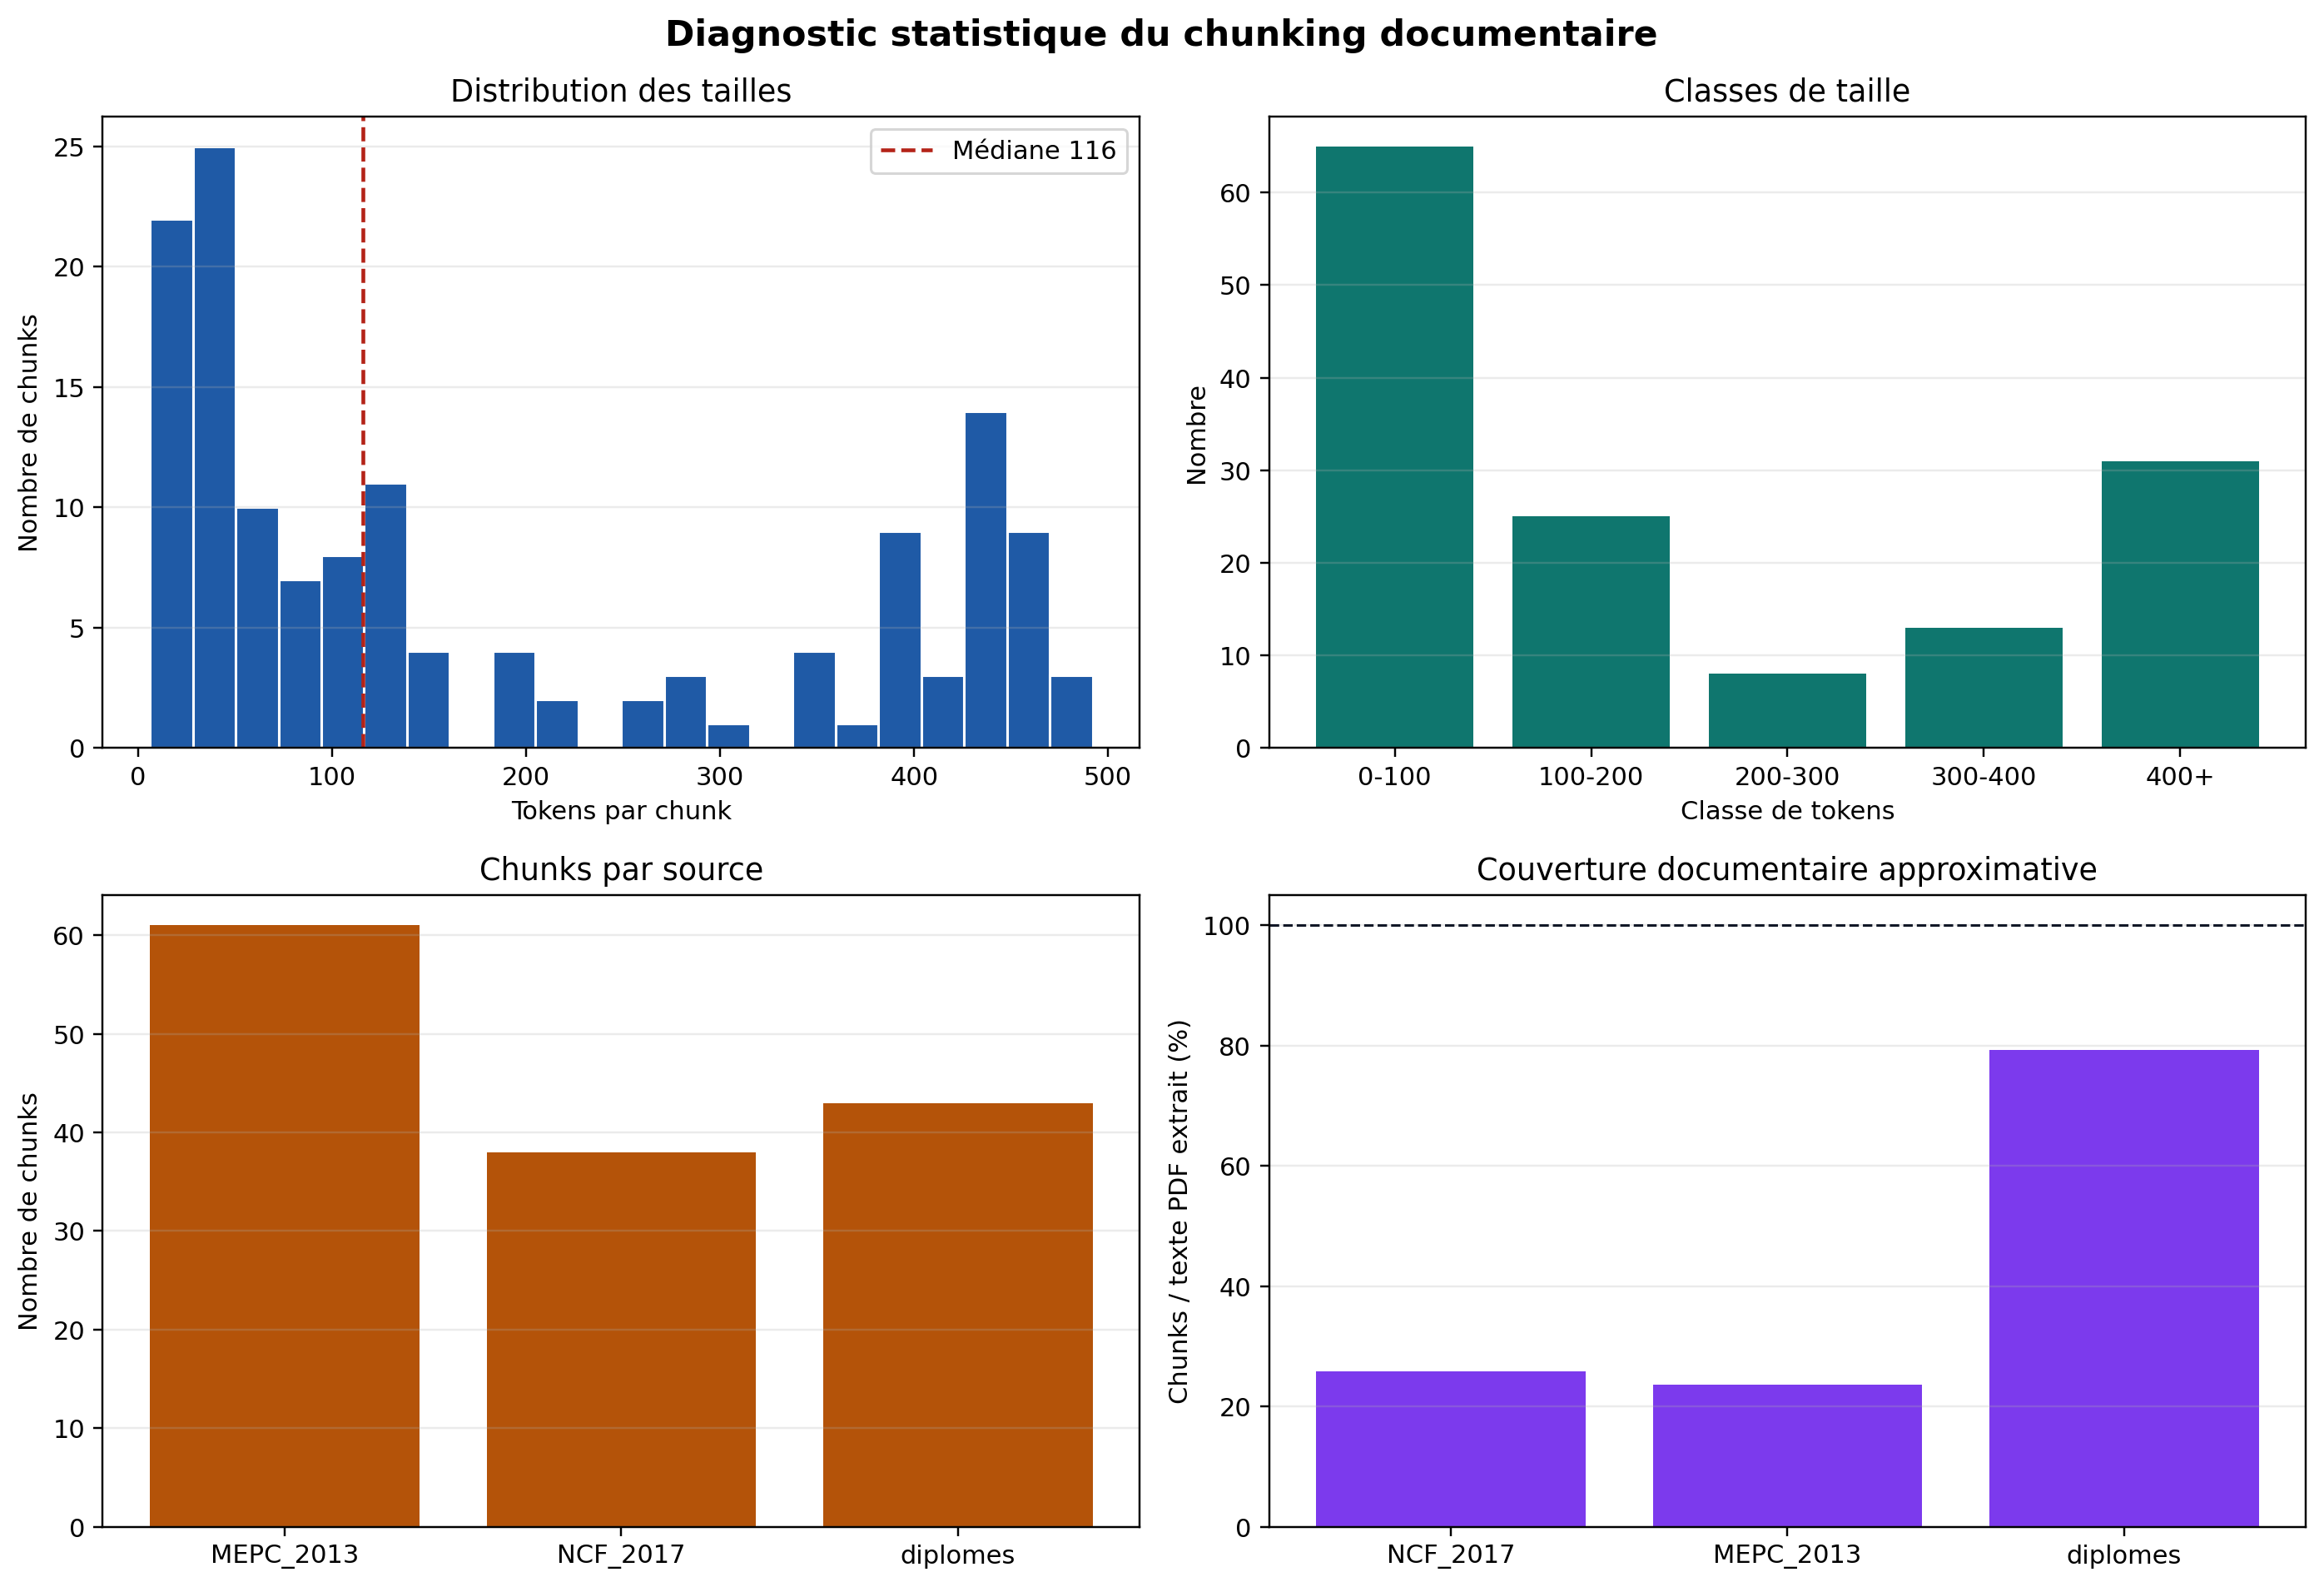
\includegraphics[width=0.5\textwidth]{figures/generated/implementation_deep_current/06_chunking_diagnostics.png}
  \source{Nos travaux, traitements Python de nettoyage et de diagnostic, à partir des données collectées du projet.}
\end{figure}

La figure~\ref{fig:implementation_chunking_diagnostics} vérifie que le pipeline produit des unités interrogeables. La médiane de 116 tokens est adaptée au retrieval : les passages sont assez courts pour être précis, mais assez longs pour conserver un contexte de section. La forte variabilité, avec un coefficient de variation de 0,91, vient de la structure des référentiels : certaines sections sont de simples intitulés, d'autres contiennent des listes ou descriptions plus longues. Ce n'est pas une erreur de traitement ; c'est un signal de surveillance. Les très petits chunks risquent d'être peu informatifs, tandis que les plus longs peuvent mélanger plusieurs idées.

\begin{figure}[H]
  \centering
  \caption{Distribution de la cohérence sémantique intra-chunk par source}
  \label{fig:implementation_chunking_coherence}
  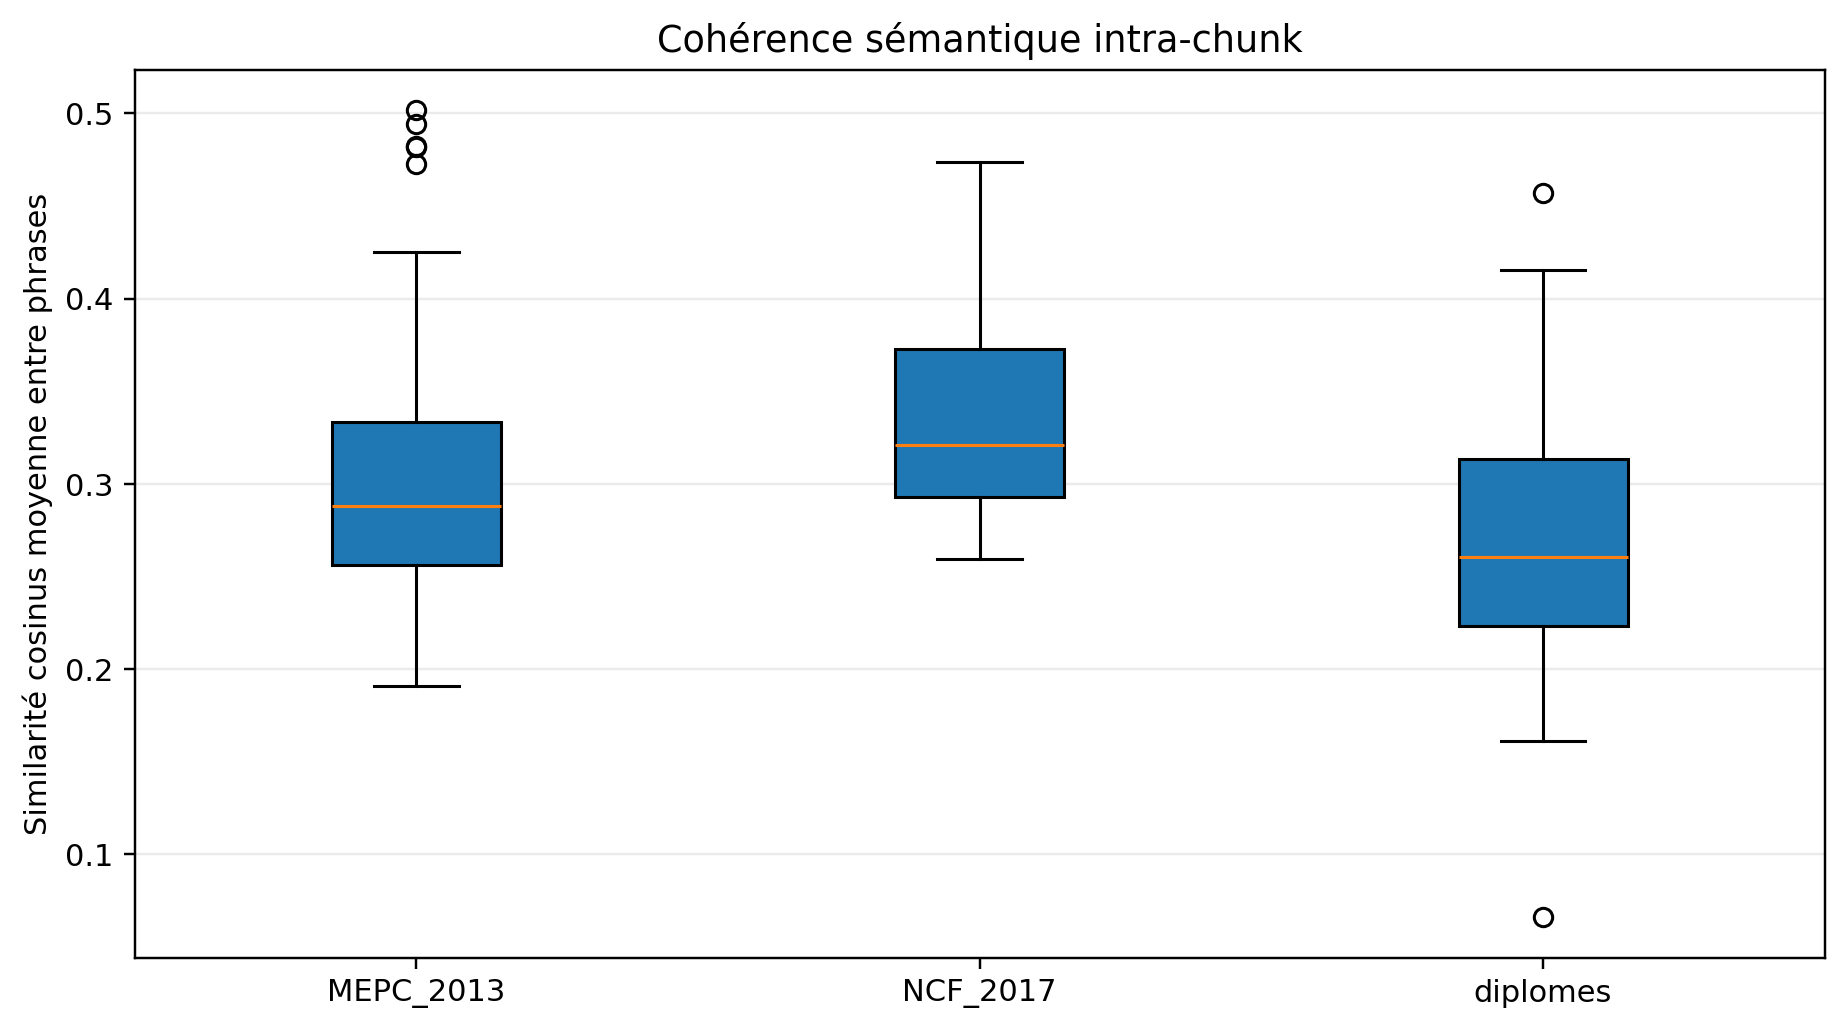
\includegraphics[width=0.4\textwidth]{figures/generated/implementation_deep_current/06_chunking_coherence_semantique.png}
  \source{Nos travaux, traitements Python de nettoyage et de diagnostic, à partir des données collectées du projet.}
\end{figure}

La figure~\ref{fig:implementation_chunking_coherence} complète cette lecture par source. La cohérence sémantique moyenne vaut 0,303 : les chunks restent exploitables, mais ils ne sont pas toujours très homogènes. Cette valeur est cohérente avec des référentiels administratifs qui combinent codes, titres, listes et descriptions courtes. L'interprétation pratique est claire : le chunking structurel respecte bien la logique réglementaire, mais les réponses RAG doivent citer les passages récupérés et éviter de surinterpréter un chunk très court ou trop composite. Les mesures détaillées sont reportées en annexe aux tableaux~\ref{tab:implementation_chunking_coverage_duplication}, \ref{tab:implementation_pgvector_chunking} et \ref{tab:implementation_chunking_coherence}.

\subsection{Index et modes de recherche mobilisés}

Les index pgvector ne sont pas seulement un détail de base de données ; ils déterminent la manière dont le workflow récupère les preuves. Trois usages sont distingués. Le premier est le rappel sémantique top-$K$ par HNSW, utilisé pour obtenir rapidement les offres, candidats, métiers ou compétences proches d'une requête. Le deuxième est le filtrage par type d'entité, indispensable pour éviter de comparer une offre avec un chunk documentaire lorsque l'outil attend une offre. Le troisième est la recherche textuelle française, utile lorsque la requête contient un terme exact que l'embedding peut diluer.

La latence observée reste compatible avec un usage interactif : la médiane vaut 30,89 ms pour un top-10 HNSW. Le maximum de 160,40 ms rappelle cependant que l'Agentic RAG doit raisonner en chaîne complète : retrieval, enrichissement Neo4j, construction du contexte et génération. Les indicateurs techniques détaillés sont donc placés en annexe aux tableaux~\ref{tab:implementation_pgvector_indicateurs} et \ref{tab:implementation_pgvector_index}. Dans le corps du chapitre, la conclusion est limitée mais suffisante : pgvector produit un vivier rapide, typé et raccordable à Neo4j.

\section{Neo4j : mémoire relationnelle du matching}

Dans le workflow, Neo4j intervient après le rappel pgvector. pgvector propose des voisins sémantiques ; Neo4j vérifie ensuite si ces voisins sont reliés par des chemins métier défendables : compétences possédées, compétences requises, métier de référence, niveau \NCF{}, secteur et localisation. Cette section montre donc comment le graphe transforme une proximité textuelle en explication contrôlable.

\subsection{Schéma, noeuds et relations mobilisés par le matching}

\begin{figure}[H]
  \centering
  \caption{Schéma logique du graphe de connaissances}
  \label{fig:implementation_schema_graphe}
  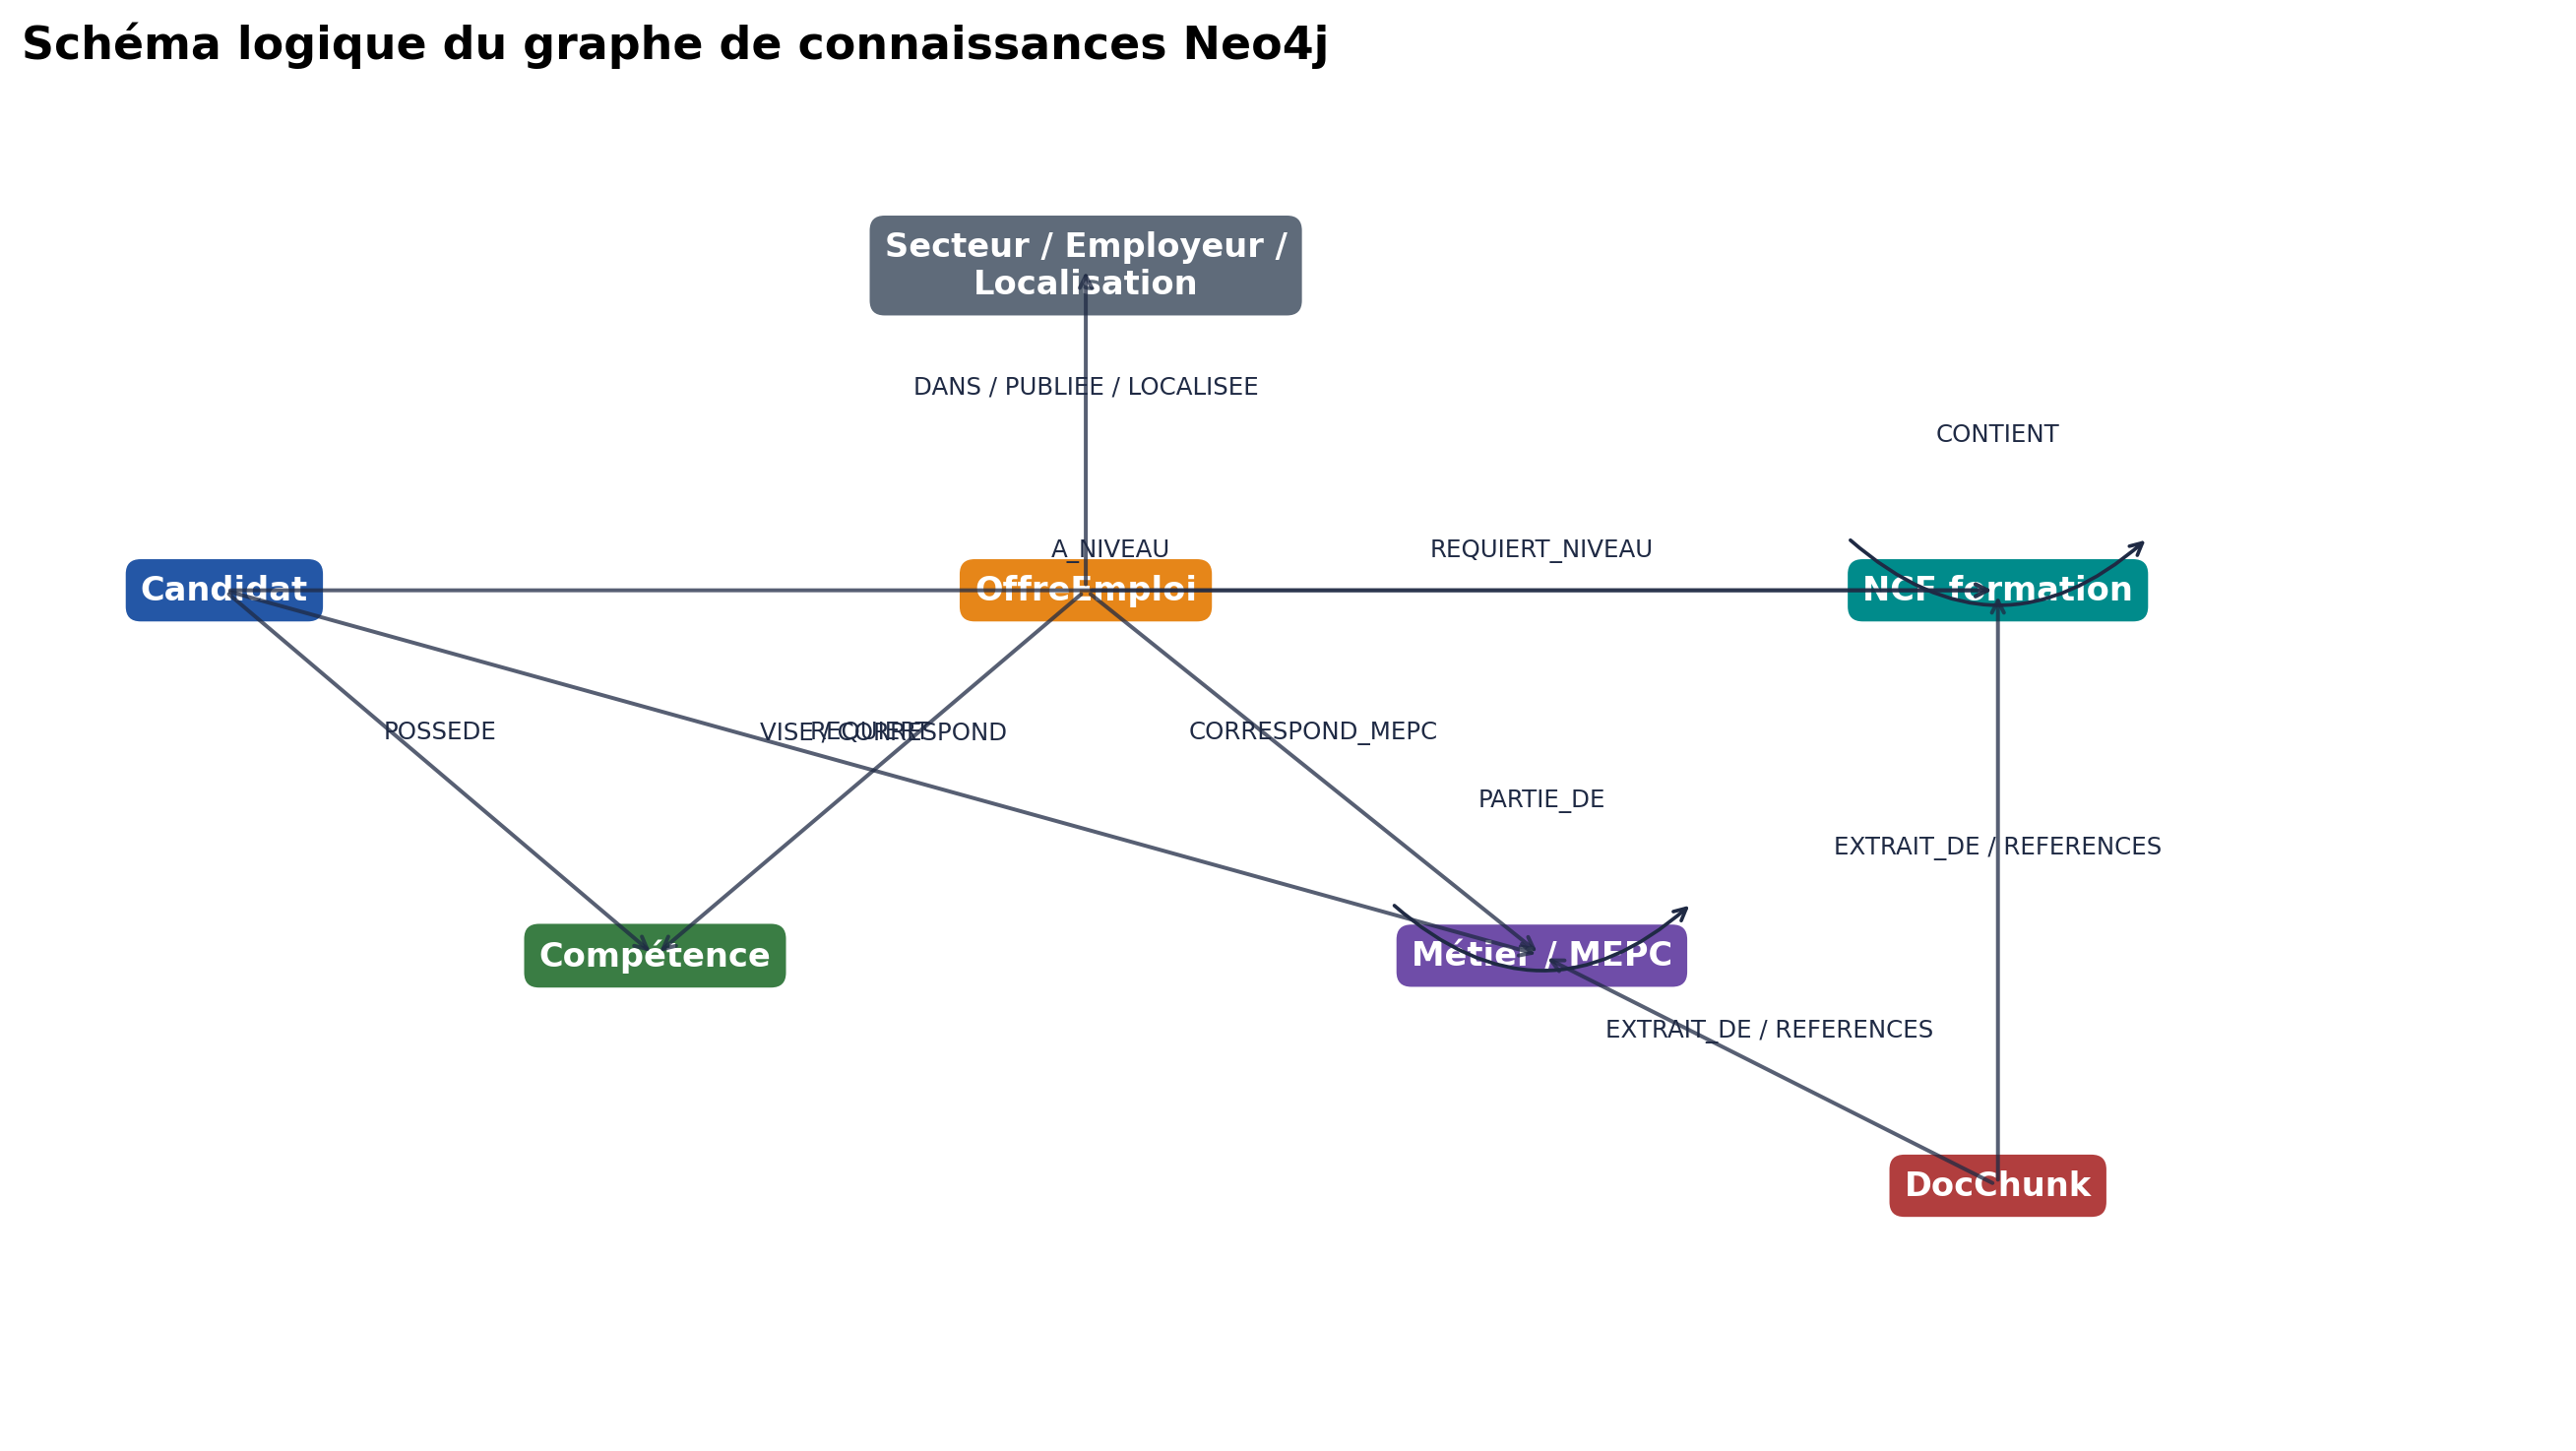
\includegraphics[width=0.3\textwidth]{figures/generated/implementation_deep_current/11_schema_graphe_connaissances.png}
  \source{Nos travaux, diagnostics Neo4j}
\end{figure}

La figure~\ref{fig:implementation_schema_graphe} donne la structure logique du graphe : les candidats et les offres sont reliés aux compétences, métiers, secteurs, localisations, niveaux \NCF{}, référentiels \MEPC{} et chunks documentaires. L'idée centrale est simple : pgvector mesure une proximité textuelle, tandis que Neo4j vérifie si cette proximité repose sur des relations métier lisibles.

\begin{figure}[H]
  \centering
  \caption{Lecture conjointe des noeuds et relations Neo4j mobilisés par le matching}
  \label{fig:implementation_neo4j_noeuds_relations}
  \begin{minipage}[t]{0.3\textwidth}
    \centering
    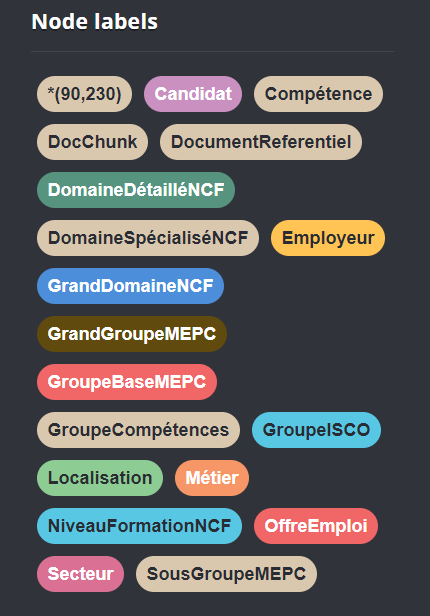
\includegraphics[width=\textwidth]{noeuds_neo4j.png}
    \caption*{\normalsize (a) Types de noeuds}
  \end{minipage}\hfill
  \begin{minipage}[t]{0.24\textwidth}
    \centering
    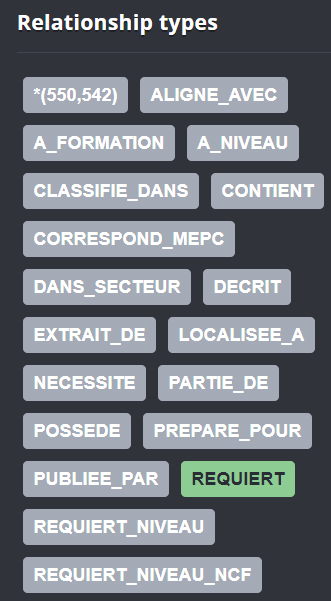
\includegraphics[width=\textwidth]{relations_neo4j.png}
    \caption*{\normalsize (b) Types de relations}
  \end{minipage}
  \source{Nos travaux, diagnostics Neo4j, à partir du graphe de connaissances emploi--compétences construit dans le projet.}
\end{figure}

La figure \ref{fig:implementation_neo4j_noeuds_relations} doit être lue en deux temps. Le panneau des noeuds indique les objets que le système manipule : \texttt{Candidat}, \texttt{OffreEmploi}, \texttt{Compétence}, \texttt{Métier}, référentiels MEPC, niveaux et domaines NCF, secteurs, employeurs, localisations et fragments documentaires. Le panneau des relations indique ce que le système sait vérifier entre ces objets : un candidat \texttt{POSSEDE} des compétences, une offre \texttt{REQUIERT} des compétences, un métier \texttt{NECESSITE} des compétences de référence, une offre est rattachée à un secteur, à un niveau, à un employeur et à une localisation. L'information utile n'est donc pas le noeud isolé, mais le couple \og objet + relation \fg{}.

La figure~\ref{fig:implementation_neo4j_noeuds_relations} précise les objets manipulés et les relations effectivement mobilisées. Une recommandation devient défendable lorsque le chemin est explicite : candidat $\rightarrow$ compétences possédées $\rightarrow$ compétences requises par l'offre, puis éventuellement métier, niveau \NCF{}, secteur ou formation de référence. Si ce chemin est absent ou porté seulement par une compétence trop générale, le graphe doit rétrograder l'offre plutôt que la justifier artificiellement.

Ces relations restent des signaux opérationnels, pas des vérités absolues. Les liens \texttt{REQUIERT} et \texttt{POSSEDE} dépendent de l'extraction et du rattachement lexical des compétences. Une compétence mal extraite ou trop générique peut donc améliorer artificiellement le score. C'est pourquoi les indicateurs de structure, de hubs et de centralité sont nécessaires avant d'utiliser Neo4j comme brique de reranking.
\subsection{Structure du graphe et risques de hubs}

\subsubsection{Taille réelle du graphe et couverture de la projection matching}

\begin{figure}[H]
  \centering
  \caption{Tableau de bord statistique du graphe Neo4j}
  \label{fig:implementation_neo4j_dashboard}
  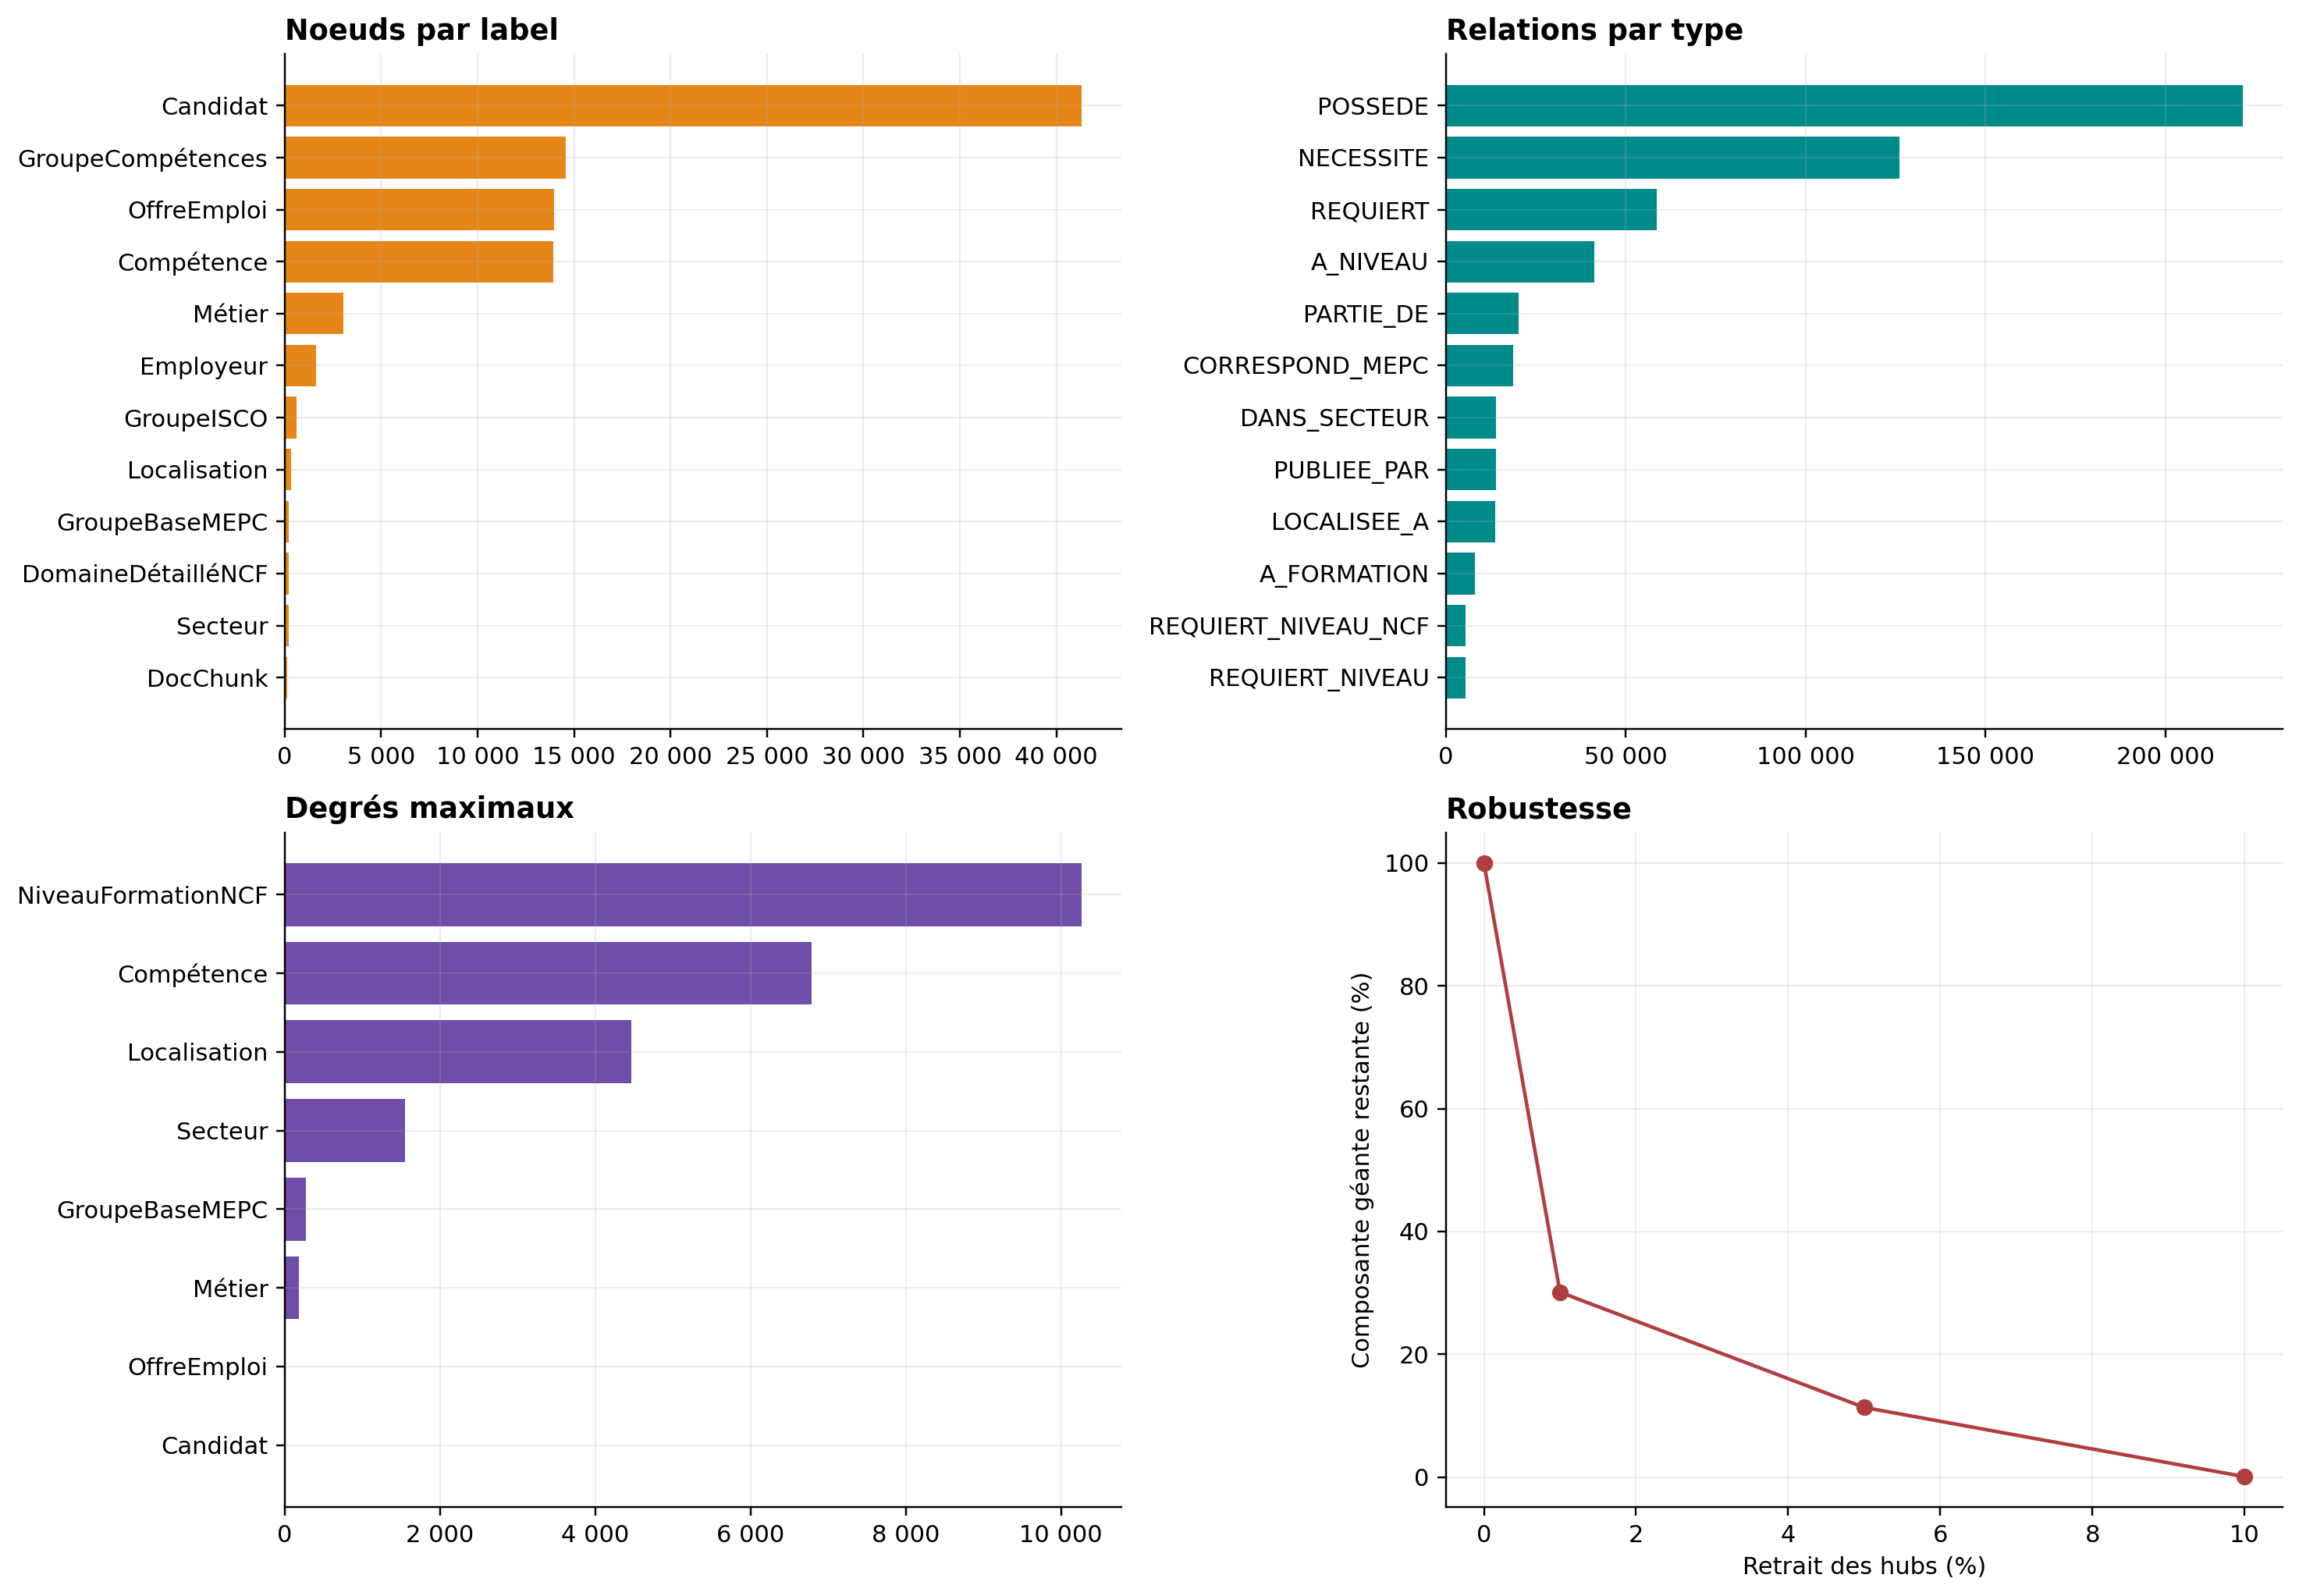
\includegraphics[width=0.5\textwidth]{figures/generated/implementation_deep_current/14_neo4j_dashboard_reseau.png}
  \source{Nos travaux, diagnostics Neo4j}
\end{figure}

La figure~\ref{fig:implementation_neo4j_dashboard} synthétise les volumes et la structure globale du graphe avant l’analyse détaillée. Elle sert ici de point d’entrée : le graphe doit d’abord être compris par ses ordres de grandeur, puis seulement par ses hubs, ses communautés et ses chemins de matching.

Le graphe complet contient 90\,230 noeuds et 550\,542 relations, répartis en 18 labels et 18 types de relations. Sa densité dirigée globale est très faible, environ $6{,}76 \times 10^{-5}$, ce qui est normal pour un graphe hétérogène de connaissances : toutes les entités n'ont pas vocation à être reliées entre elles. Cette faible densité ne signifie donc pas que le graphe est pauvre ; elle signifie qu'il encode des relations spécialisées plutôt qu'un réseau où tout serait connecté à tout.

Pour analyser la partie réellement mobilisée par le matching, une projection non orientée a été construite à partir des relations \texttt{POSSEDE}, \texttt{REQUIERT}, \texttt{NECESSITE}, \texttt{CORRESPOND\_MEPC}, \texttt{A\_NIVEAU}, \texttt{REQUIERT\_NIVEAU}, \texttt{DANS\_SECTEUR} et \texttt{LOCALISEE\_A}. Cette projection contient 72\,516 noeuds et 499\,080 arêtes ; elle forme une seule composante connexe. Ce résultat est important : les entités utiles au matching ne sont pas dispersées en sous-graphes indépendants, elles appartiennent à un même réseau de propagation candidat--offre--compétence. En pratique, cela permet au GraphRAG de construire des chemins courts entre un profil, une offre, une compétence, un métier ou un niveau de formation.
La composition détaillée des noeuds et relations est reportée en annexe (figure~\ref{fig:implementation_neo4j_composition}).

Les principaux labels sont \texttt{Candidat} avec 41\,298 noeuds, \texttt{GroupeCompétences} avec 14\,579 noeuds, \texttt{OffreEmploi} avec 13\,957 noeuds, \texttt{Compétence} avec 13\,939 noeuds et \texttt{Métier} avec 3\,039 noeuds. Les cinq premiers labels concentrent 96,21\,\% des noeuds. Cette structure est cohérente avec l'objectif métier : le graphe est d'abord un graphe d'appariement, non un graphe encyclopédique. Le risque statistique est clair : si le score de recommandation n'est pas normalisé, les familles très représentées peuvent dominer la recherche au détriment de signaux plus spécifiques comme le métier, le niveau ou le secteur.

Cette structure impose toutefois une lecture prudente. Comme les relations de compétences dominent fortement, le score final dépend beaucoup de leur qualité. Si une offre n'a pas de relation \texttt{REQUIERT}, Neo4j ne peut pas calculer correctement la couverture de compétences. Si une compétence générique devient trop connectée, elle peut créer un hub peu discriminant. L'apport du graphe existe donc à condition de contrôler la complétude et la précision des relations.

\subsubsection{Noeuds très connectés : signal utile ou bruit de popularité}

La distribution complète des degrés est placée en annexe (figure~\ref{fig:implementation_neo4j_distribution_degres}). La distribution des degrés est fortement asymétrique. L'estimation exploratoire d'une loi de puissance sur la queue de distribution donne un exposant compris entre 1,40 et 2,51 selon le seuil $x_{\min}$ retenu. Ce n'est pas une preuve formelle de loi de puissance, mais un diagnostic utile : le graphe comporte bien des hubs. Dans un système de recommandation, ces hubs doivent être traités avec prudence. Une compétence très connectée n'est pas automatiquement discriminante ; elle peut simplement être générique, très fréquente ou issue d'un référentiel large.

Le tableau d'hétérogénéité des degrés par famille de noeuds est reporté en annexe (tableau~\ref{tab:implementation_neo4j_degres}). Les degrés moyens montrent une forte hétérogénéité. Les noeuds \texttt{NiveauFormationNCF} ont un degré moyen de 5\,812,56, parce que neuf niveaux seulement absorbent une grande partie des relations candidat--niveau et offre--niveau. Les \texttt{GroupeBaseMEPC}, les \texttt{Secteur}, les \texttt{Métier}, les \texttt{Localisation} et les \texttt{Compétence} jouent aussi un rôle de concentration. Cette hétérogénéité est une force pour l'explication, mais une faiblesse pour le scoring si elle n'est pas normalisée : le graphe peut favoriser des noeuds populaires au lieu de noeuds réellement informatifs.

\subsubsection{Compétences pivots selon degré, PageRank et intermédiarité}

\begin{figure}[H]
  \centering
  \caption{Centralités des compétences : degré, PageRank et intermédiarité approximée}
  \label{fig:implementation_neo4j_centralites_competences}
  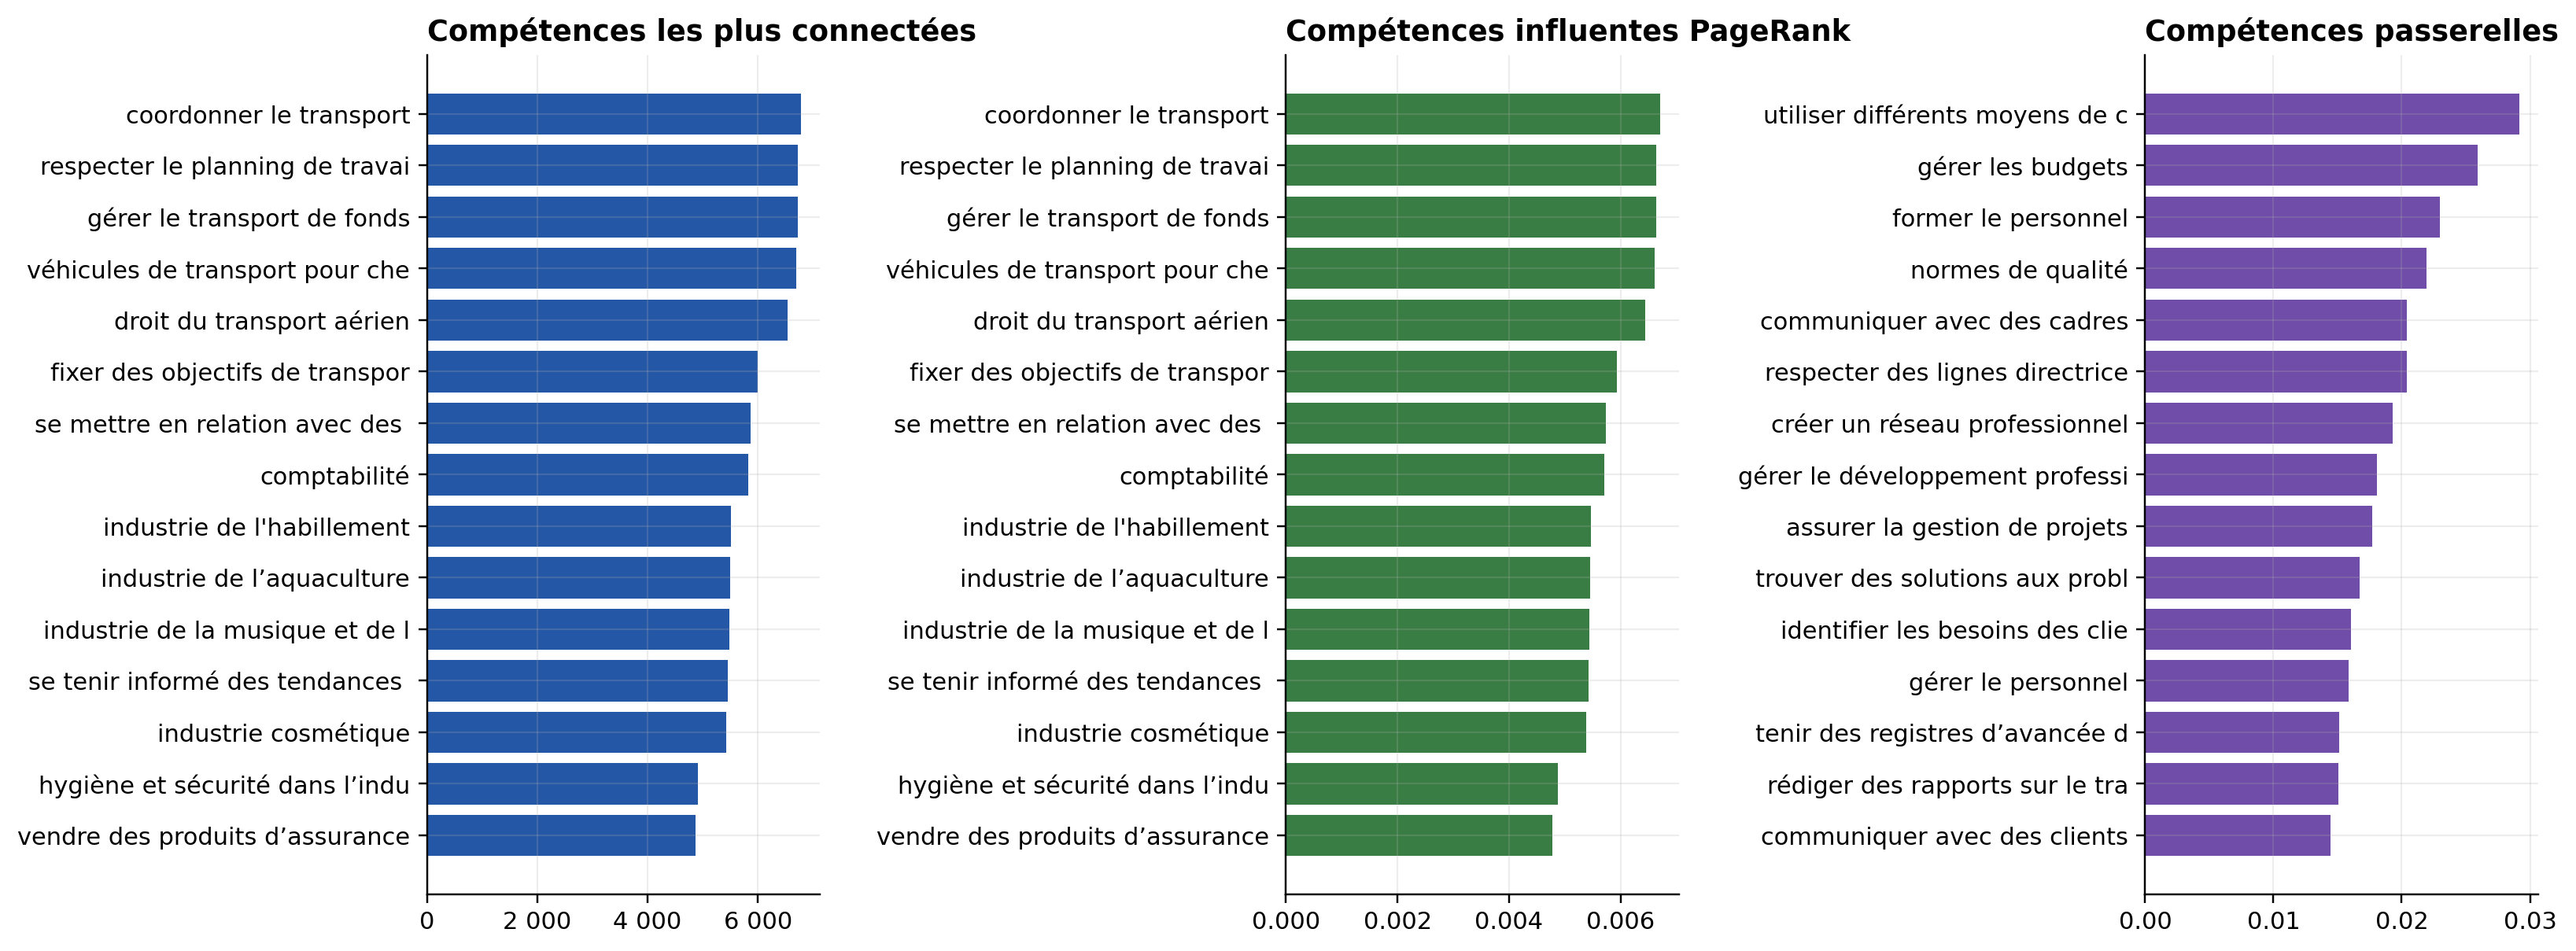
\includegraphics[width=0.94\textwidth]{figures/generated/implementation_deep_current/15_neo4j_centralites_competences.png}
  \source{Nos travaux, diagnostics Neo4j, à partir du graphe de connaissances emploi--compétences construit dans le projet.}
\end{figure}

Les centralités donnent trois lectures complémentaires. La centralité de degré et le PageRank identifient surtout les compétences les plus connectées, par exemple \og coordonner le transport \fg{}, \og respecter le planning de travail dans les transports \fg{}, \og gérer le transport de fonds \fg{} et \og comptabilité \fg{}. L'intermédiarité approximée, calculée sur le sous-graphe des noeuds de plus fort degré, fait ressortir d'autres compétences : \og utiliser différents moyens de communication \fg{}, \og gérer les budgets \fg{}, \og former le personnel \fg{}, \og normes de qualité \fg{} et \og assurer la gestion de projets \fg{}. Ces dernières sont plus intéressantes pour la recommandation, car elles jouent un rôle de passerelle entre plusieurs familles de métiers.

Les exemples de compétences centrales selon les métriques de graphe sont placés en annexe (tableau~\ref{tab:implementation_neo4j_centralites}).

La distinction entre degré, PageRank et intermédiarité est importante. Un noeud à fort degré est fréquent ; il peut donc être utile, mais peu discriminant. Un noeud avec PageRank élevé structure le réseau parce qu'il est relié à des noeuds eux-mêmes importants. Un noeud avec intermédiarité élevée sert de passerelle entre plusieurs zones du graphe. Pour le \textit{skill gap}, ces compétences passerelles sont particulièrement utiles : elles indiquent des compétences transversales qui peuvent rapprocher plusieurs trajectoires professionnelles. Dans le moteur hybride, cela justifie de ne pas traiter toutes les compétences manquantes de la même manière.

\subsubsection{Communautés Louvain et robustesse aux hubs}

Les communautés Louvain et distances sont détaillées en annexe (figure~\ref{fig:implementation_neo4j_communautes}).

La détection de communautés a été réalisée avec Louvain sur un échantillon pondéré de la composante géante, enrichi par les noeuds de plus fort degré afin de conserver l'ossature du réseau. Elle identifie 100 communautés dans la projection analysée. Ce résultat ne doit pas être vendu comme une typologie définitive des métiers ; il sert à vérifier que le graphe contient des regroupements relationnels exploitables. La distance moyenne échantillonnée dans la composante géante vaut 4,10 sauts, avec une médiane de 4. En pratique, cela signifie qu'un candidat, une offre, une compétence ou un métier peut être relié au reste du réseau par quelques relations seulement, ce qui rend le GraphRAG opérationnel pour produire des chemins explicatifs courts.

Le test de robustesse après retrait des hubs est reporté en annexe (figure~\ref{fig:implementation_neo4j_robustesse}).

Le test de robustesse retire successivement les 1\,\%, 5\,\% et 10\,\% de noeuds les plus centraux selon le degré, puis mesure la taille de la composante géante restante. Ce test est sévère, car il cible les hubs au lieu de supprimer des noeuds au hasard. Son intérêt est de mesurer la dépendance du graphe à quelques entités très connectées. Si la composante géante s'effondre fortement après retrait des hubs, cela signifie que le système dépend excessivement de compétences ou niveaux génériques. Dans ce cas, le reranking doit pénaliser les hubs trop peu discriminants et valoriser les compétences spécifiques.

\subsubsection{Skill gap observé entre profils et offres}

Les compétences moyennes par objet métier sont visualisées en annexe (figure~\ref{fig:implementation_neo4j_competences_entites}).

L'analyse métier confirme le rôle pivot des compétences. Une offre exige en moyenne 4,19 compétences, avec une médiane de 6. Un candidat possède en moyenne 5,36 compétences, avec une médiane de 6. Les métiers sont beaucoup plus riches : 41,48 compétences en moyenne et 37 en médiane, parce qu'ils agrègent des exigences de référentiel. Cette différence est saine : l'offre et le candidat portent un signal opérationnel court ; le métier porte un contexte plus large qui sert à l'enrichissement, à l'explication et à la montée en compétences.

%\begin{table}[H]
%  \centering
%  \caption{Nombre moyen de compétences par objet métier}
%  \label{tab:implementation_neo4j_competences_moyennes}
%  \tableStyleStart
%  \begin{tabularx}{0.88\textwidth}{Xrrrr}
%    \rowcolor{darkblue}
%    \tabheader{Objet} & \tabheader{Effectif} & \tabheader{Moyenne} & \tabheader{Médiane} & \tabheader{p90} \\
%    \midrule
%    Offre & 13\,957 & 4,19 & 6 & 6 \\
%    Candidat & 41\,298 & 5,36 & 6 & 6 \\
%    Métier & 3\,039 & 41,48 & 37 & 70 \\
%    \bottomrule
%  \end{tabularx}
%  \tableStyleEnd
%  \source{\texttt{17\_neo4j\_competences\_moyennes.csv}}
%\end{table}

La distribution détaillée du skill gap candidat--offre est renvoyée en annexe (figure~\ref{fig:implementation_neo4j_skill_gap}).

Le \textit{skill gap} a été mesuré sur un échantillon de couples candidat--offre en comparant les compétences \texttt{REQUIERT} de l'offre aux compétences \texttt{POSSEDE} du candidat. Le déficit moyen est de 5,32 compétences, avec une médiane de 6 ; seulement 12,33\,\% des couples échantillonnés ont un déficit inférieur ou égal à trois compétences. Ce résultat est sévère, mais utile : le graphe ne dit pas que la majorité des candidats sont immédiatement compatibles avec une offre prise au hasard. Il montre au contraire que le matching doit sélectionner, filtrer et reranker. C'est précisément la raison d'être du moteur hybride : utiliser pgvector pour présélectionner des couples plausibles, puis Neo4j pour mesurer finement les compétences acquises, manquantes et passerelles.

L'interprétation opérationnelle est directe. Lorsque le déficit est faible, l'offre peut être considérée comme accessible ou proche. Lorsque le déficit est moyen, la recommandation doit être accompagnée d'un plan de montée en compétences. Lorsque le déficit est élevé, le système doit éviter de présenter l'offre comme immédiatement réaliste. Le graphe apporte donc une information que la similarité vectorielle seule ne fournit pas : il distingue la ressemblance textuelle d'une compatibilité professionnelle argumentée.

%\begin{figure}[H]
 % \centering
%  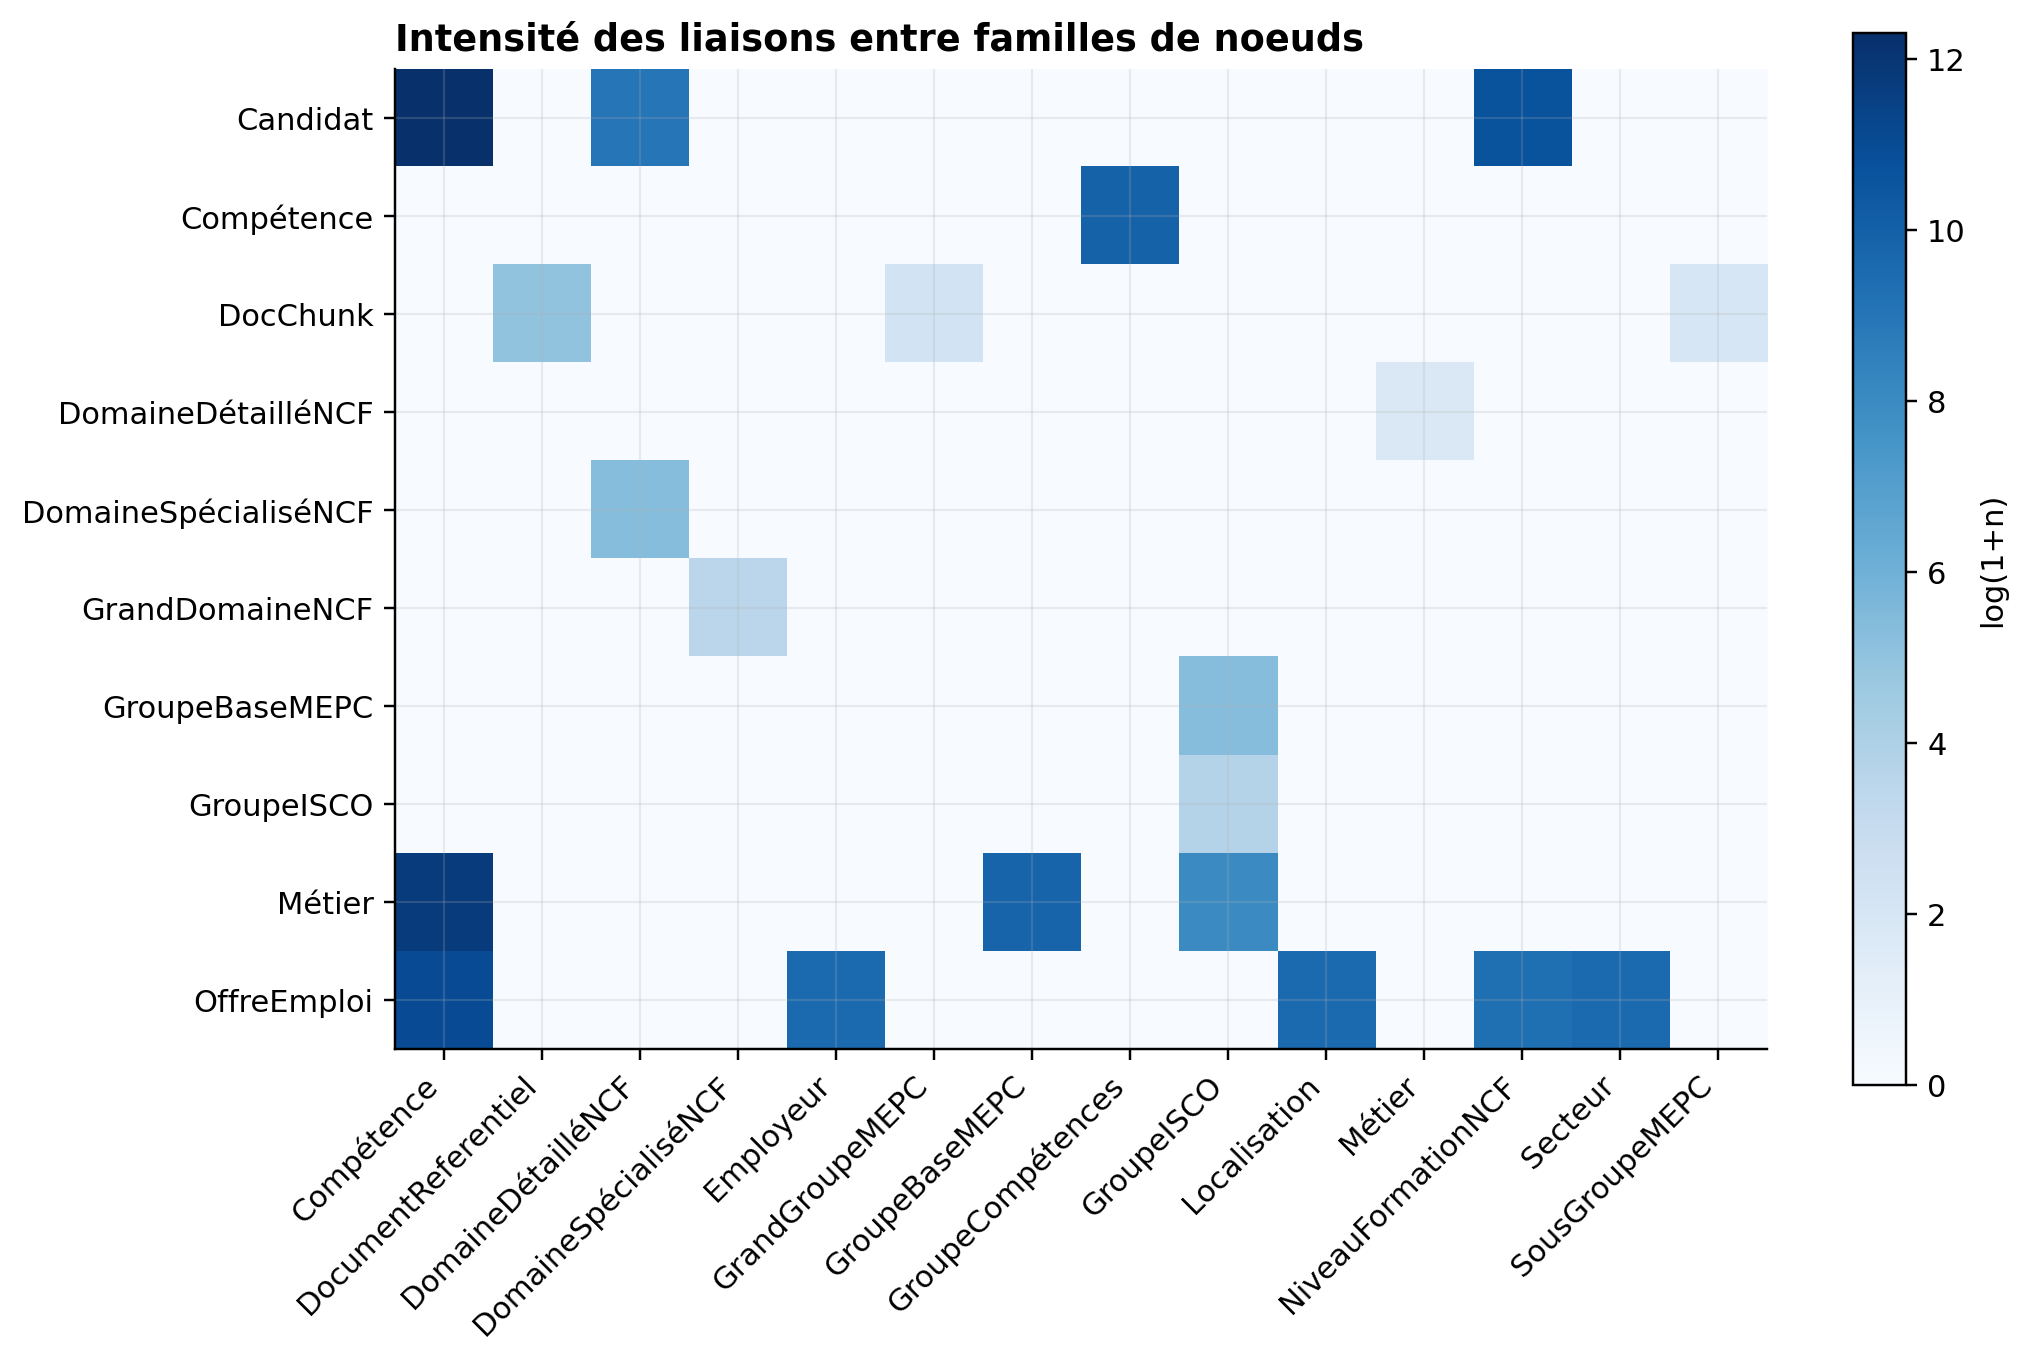
\includegraphics[width=0.86\textwidth]{figures/generated/implementation_deep_current/10_neo4j_matrice_liaisons.png}
%  \caption{Matrice des liaisons entre familles de noeuds}
%  \label{fig:implementation_neo4j_matrice}
%  \source{\texttt{08\_neo4j\_patterns\_top.csv}}
%\end{figure}

%La matrice des liaisons confirme que le graphe n'est pas seulement une collection de tables importées. Les motifs les plus importants sont les chemins candidat--compétence--offre portés par \texttt{POSSEDE} et \texttt{REQUIERT}, avec respectivement 221\,413 relations candidat--compétence et 58\,519 relations offre--compétence, ainsi que 126\,051 relations métier--compétence portées par \texttt{NECESSITE}. Ces chemins sont directement exploitables : ils permettent de calculer un taux de couverture des compétences, d'identifier les compétences manquantes, de rattacher l'offre à un métier et de proposer une trajectoire de montée en compétences.

La conclusion à retenir est donc précise. Le graphe est riche parce qu'il relie les objets utiles au recrutement ; il est déséquilibré parce que certaines compétences et certains métiers concentrent beaucoup de relations ; il est décisionnel parce qu'il modifie le classement produit par pgvector ; il reste imparfait parce que les liens de compétences dépendent de la qualité de l'extraction et du rattachement lexical. Cette nuance est importante : Neo4j améliore l'explicabilité et le reranking, mais il ne doit pas être présenté comme une garantie automatique de vérité métier.

\section{Score hybride et reranking des recommandations}

Le moteur hybride constitue le coeur décisionnel du système. Sans lui, l'application ne serait qu'un chatbot branché sur une recherche vectorielle. L'implémentation suit une logique en trois temps : pgvector présélectionne un ensemble d'offres candidates, Neo4j enrichit chaque couple candidat--offre avec des signaux relationnels, puis un score hybride réordonne les offres avant la génération. Le classement final n'est donc pas directement le score de similarité textuelle ; c'est un arbitrage pondéré entre le score pgvector et le score Neo4j, calibré ensuite par Optuna.

\subsection{Formalisation du score hybride}

Le score hybride utilisé pour le reranking ne doit pas être présenté comme une addition de nombreux critères indépendants. Dans la version évaluée ici, il combine deux signaux seulement. Le premier vient de pgvector : il mesure la proximité sémantique entre le profil ou la requête et l'offre candidate. Le second vient de Neo4j : il mesure la compatibilité relationnelle, principalement à travers la couverture des compétences requises par l'offre et possédées par le candidat. La formulation retenue est donc :

\[
S_{\text{hybride}} =
\alpha S_{\text{pgvector}} + \beta S_{\text{Neo4j}},
\quad \alpha+\beta=1
\]

\noindent où $S_{\text{pgvector}}$ correspond à la colonne \texttt{score\_sem} et $S_{\text{Neo4j}}$ à la colonne \texttt{taux\_match}. Cette écriture est volontairement simple : pgvector répond à la question \og les textes se ressemblent-ils ? \fg{}, alors que Neo4j répond à la question \og les compétences exigées sont-elles couvertes ? \fg{}. Les autres informations du graphe, comme le niveau NCF, le secteur ou la localisation, restent utiles pour l'explication et les verdicts, mais elles ne sont pas ajoutées comme poids autonomes dans cette calibration. Sinon, le score deviendrait difficile à défendre statistiquement et risquerait de compter plusieurs fois le même signal métier.

\begin{figure}[H]
  \centering
  \caption{Distribution comparée des scores pgvector et Neo4j utilisés dans le reranking}
  \label{fig:implementation_distribution_scores_hybrides}
  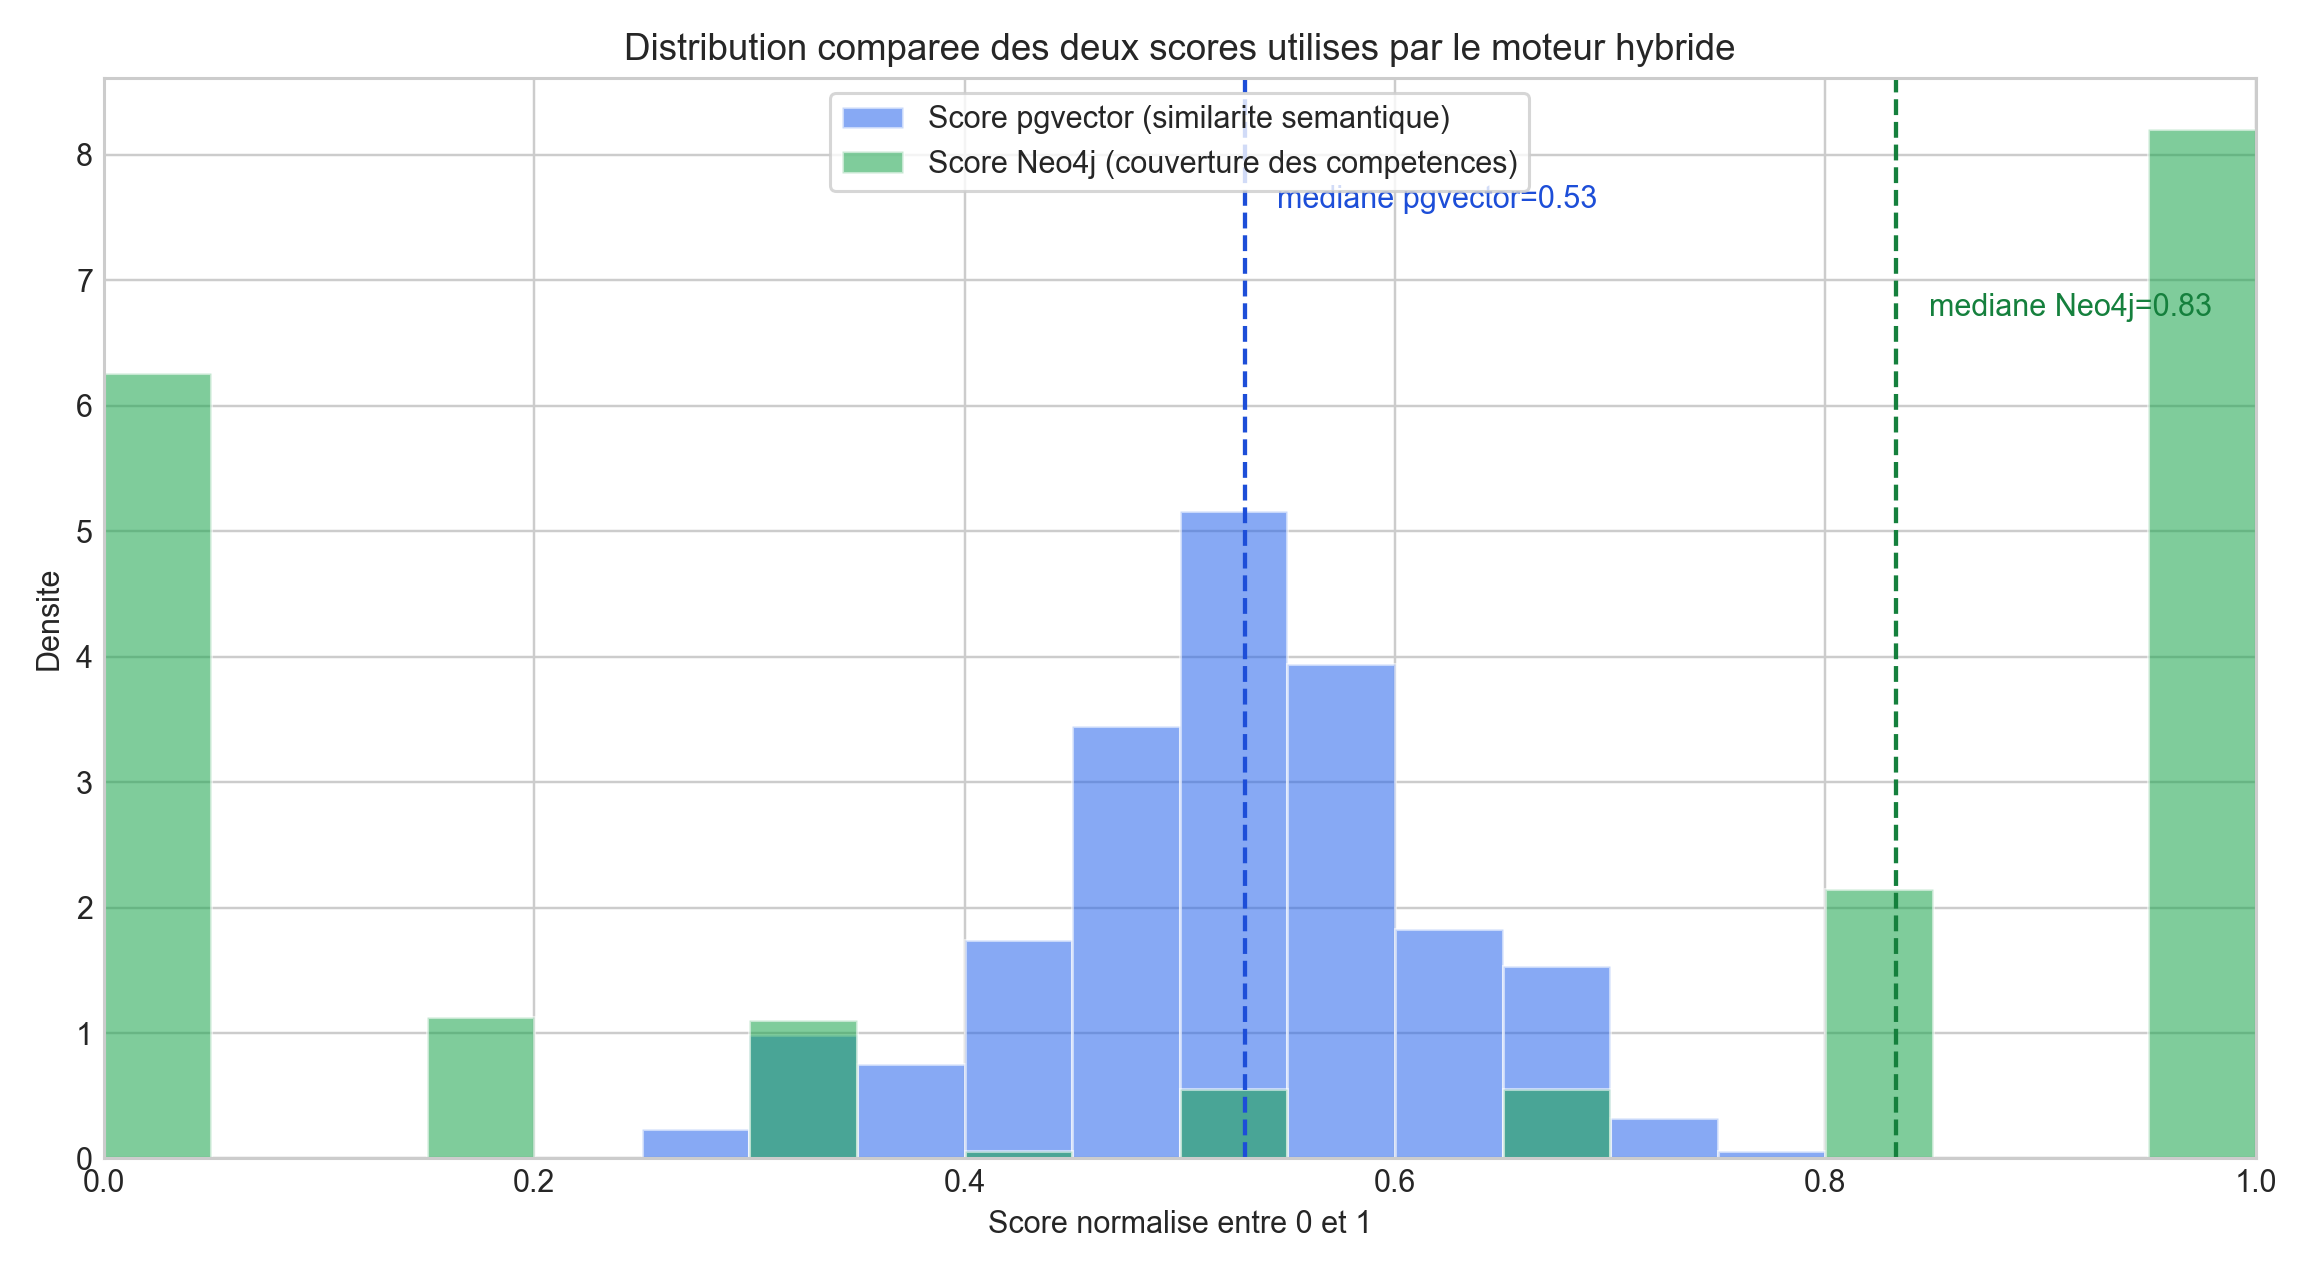
\includegraphics[width=0.55\textwidth]{figures/generated/implementation_deep_current/13_distribution_scores_pgvector_neo4j.png}
  \source{Nos travaux, diagnostics PostgreSQL--pgvector, à partir des embeddings}
\end{figure}

La figure \ref{fig:implementation_distribution_scores_hybrides} montre que les deux scores n'ont pas le même comportement. Le score pgvector est continu et relativement concentré : sa moyenne vaut 0,5225 et sa médiane 0,5304 sur les 690 couples candidat--offre évalués. Le score Neo4j est plus discontinu : sa moyenne vaut 0,5606, sa médiane 0,8330, mais 31,30\,\% des couples ont un score nul. Cette différence est normale. pgvector renvoie presque toujours une proximité textuelle, même moyenne ; Neo4j est plus sévère, car une offre peut être textuellement proche tout en n'ayant aucune compétence requise couverte par le candidat.

\begin{table}[H]
  \centering
  \caption{Résultats de calibration des poids du score hybride}
  \label{tab:implementation_moteur_hybride_score}
  \tableStyleStart
  \normalsize
  \setlength{\tabcolsep}{3pt}
  \renewcommand{\arraystretch}{1.16}
  \begin{tabularx}{0.98\textwidth}{>{\raggedright\arraybackslash}X
      >{\raggedright\arraybackslash}p{2.55cm}
      >{\centering\arraybackslash}p{1.75cm}
      >{\centering\arraybackslash}p{1.65cm}
      >{\centering\arraybackslash}p{2.05cm}}
    \rowcolor{darkblue}
    \tabheader{Objectif optimisé} &
    \tabheader{Outil} &
    \tabheader{$\alpha$ Sem} &
    \tabheader{$\beta$ Neo4j} &
    \tabheader{NDCG@10} \\
    \midrule
    NDCG@10 & Neo4j seul & 0,0000 & 1,0000 & 0,9697 \\
    \makecell[l]{$(\text{NDCG@10}+\text{Recall@10}$\\$+\text{Precision@10})/3$} & Neo4j seul & 0,0000 & 1,0000 & 0,9697 \\
    \makecell[l]{$(\text{MRR@10}+\text{Precision@10})/2$} & Mixte Optuna & 0,6615 & 0,3385 & 0,9674 \\
    \bottomrule
  \end{tabularx}
  \tableStyleEnd
  \source{Nos travaux, traitements Python de nettoyage et de diagnostic, à partir des données collectées du projet.}
\end{table}

La calibration Optuna a été réalisée avec un \texttt{TPESampler}, 500 essais et une graine fixée à 42. Lorsque l'objectif est de maximiser le NDCG@10, le meilleur jeu retenu donne tout le poids au score Neo4j : $\alpha=0$ et $\beta=1$. Ce résultat ne signifie pas que pgvector est inutile. Il signifie que, sur le sous-ensemble déjà récupéré par pgvector, le reclassement est mieux ordonné lorsque la compatibilité graphe domine. La bonne lecture est donc séquentielle : pgvector sert à constituer le vivier de candidats plausibles ; Neo4j sert ensuite à départager ces candidats par couverture de compétences. Pour un objectif davantage centré sur le rang exact de la première bonne offre, le critère $(\text{MRR@10}+\text{Precision@10})/2$ retient au contraire un mélange, avec 0,6615 pour pgvector et 0,3385 pour Neo4j. Le choix final dépend donc du besoin applicatif : maximiser la qualité du top 10 ou privilégier la première recommandation.
\subsection{Effet du reranking hybride}

L'effet du reranking se mesure à deux niveaux. Le premier niveau regarde les rangs des couples candidat--offre déjà présents dans le vivier récupéré par pgvector. Le second niveau regarde les métriques de ranking lorsque l'on compare le système \texttt{pgvector\_only} au système \texttt{pgvector\_plus\_graph}. Cette distinction est importante : Neo4j ne remplace pas le retrieval vectoriel, il intervient après lui pour réordonner les offres candidates.

La figure \ref{fig:implementation_effet_reranking_neo4j} montre un effet net du graphe sur l'ordre des résultats. Sur les 690 couples évalués, 59,86\,\% gagnent des positions après reranking, 13,77\,\% perdent des positions et 26,38\,\% restent au même rang. Le gain moyen est de 4,01 rangs, avec une médiane de 1 rang et un maximum de 28 rangs. Cette moyenne ne doit pas être interprétée comme une amélioration automatique de chaque offre : elle indique que le score Neo4j change réellement l'ordre produit par pgvector, en remontant surtout les offres dont les compétences requises sont mieux couvertes.

\begin{figure}[H]
  \centering
  \caption{Effet du reranking Neo4j sur les métriques et les déplacements de rang}
  \label{fig:implementation_effet_reranking_neo4j}
  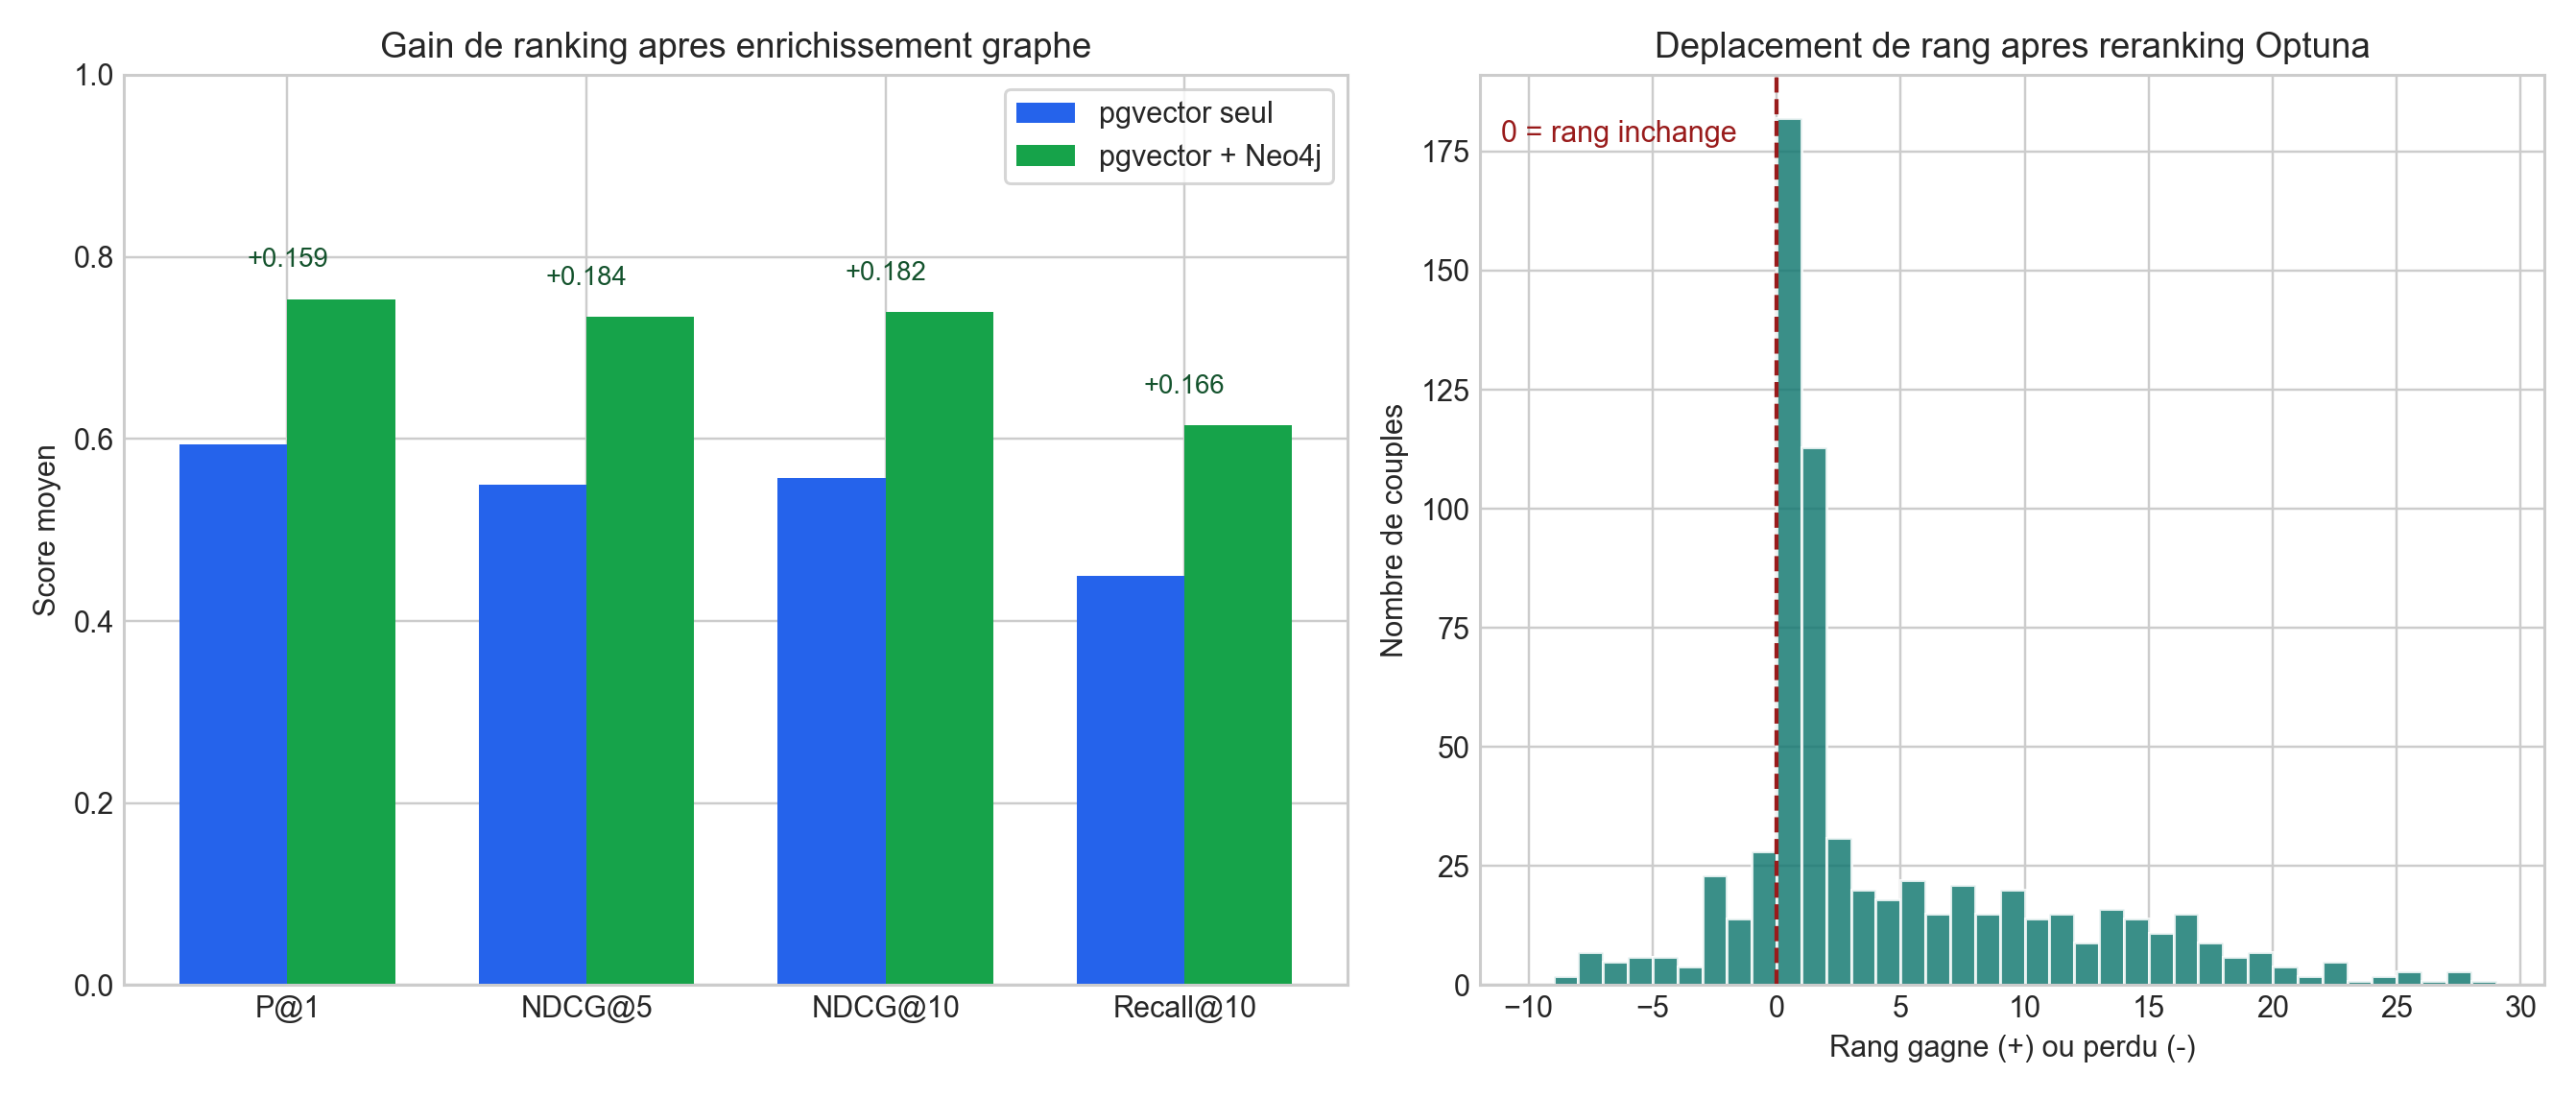
\includegraphics[width=0.94\textwidth]{figures/generated/implementation_deep_current/13_effet_reranking_pgvector_neo4j.png}
  \source{Nos travaux, diagnostics PostgreSQL--pgvector, à partir des embeddings}
\end{figure}
Le résumé détaillé des déplacements de rang après reranking est placé en annexe (tableau~\ref{tab:implementation_moteur_hybride_scores}).

L'ablation confirme ensuite que ces déplacements ne sont pas seulement cosmétiques. Sur 69 requêtes évaluées, l'ajout du graphe augmente la précision@1 de 0,5942 à 0,7536, le NDCG@5 de 0,5495 à 0,7339, le NDCG@10 de 0,5575 à 0,7392 et le recall@10 de 0,4491 à 0,6147. Le hit rate@10 reste identique à 0,9420 : cela signifie que les éléments pertinents sont souvent déjà présents dans le vivier pgvector, mais que Neo4j les ordonne mieux. C'est exactement le rôle attendu du reranking : ne pas refaire la recherche depuis zéro, mais transformer une liste plausible en liste mieux priorisée.

La conclusion doit rester stricte. Le reranking hybride améliore le classement dans ce protocole, mais la pertinence utilisée est un proxy construit à partir de métadonnées normalisées et non une annotation humaine indépendante. Le résultat est donc une preuve opérationnelle de cohérence interne, pas encore une preuve définitive de satisfaction recruteur ou candidat. Pour défendre le système en production, il faudra compléter cette évaluation par des jugements humains ou des retours d'usage.

\section*{Conclusion}

Le chapitre a suivi le workflow réel du système. Les données nettoyées alimentent d'abord l'encodeur ; l'encodeur produit les vecteurs ; pgvector construit le vivier de retrieval ; Neo4j vérifie les relations métier ; le score hybride rerange les offres candidates. Cette chaîne évite de confier toute la décision au \LLM{} : la génération intervient après la récupération, l'enrichissement relationnel et le scoring.La conclusion d'implémentation est donc précise. Le système est opérationnel parce que ses briques sont raccordées : données normalisées, modèle d'embeddings spécialisé, mémoire vectorielle, graphe de connaissances et reranking hybride. Il reste cependant dépendant de la qualité des données scrapées, de la complétude des compétences et de la validité des relations Neo4j. Le chapitre suivant évalue justement ce que ces choix apportent au retrieval, au classement et à la génération de la recommandation.
